% Chapter 1
\chapter{Tests performed} % Main chapter title

\label{sec:tests} % For referencing the chapter elsewhere, use \ref{Chapter1} 

\section{Test model: lung cancer}

\begin{itemize}
	\item Total of 9 matrices (one per age group: 35-39, 40-44, …, 75-79).
	\item 7 health states: healthy, stages I-II, stage IIIa, stage IIIb, LC survival, death from LC, death from other causes → 7x7 matrices. Sometimes the LC survival state is excluded from the calibration resulting in 6x6 matrices.
	\item Matrices represent monthly steps in the simulation. Since they are applied for 5-year groups, each matrix is used in 5 * 12 = 60 iterations in the model.
	\item A simplified calibration can be performed without running the model, only the matrices are used. This is a fast approximation since we are not considering some factors of the full model (e.g. prevalence of smoking):
	\begin{itemize}
		\item LC survival state is excluded → 6x6 matrices
		\item From the 6x6=36 probabilities per matrix, only 11 probabilities are allowed to change. The rest are either constant (zeroes, ones) or one minus the sum of the rest of the row.
		\item The error measurement is a weighted sum of the absolute differences of the LC incidence, LC mortality and mortality from other causes. The weights are 0.45, 0.45 and 0.10 respectively.
	\end{itemize}
\end{itemize}

\section{Simplified calibration}
\subsection{1 matrix}

\begin{itemize}
	\item Source file: models/lung/calibration\_wrapper.R (N\_MATRICES set to 1)
	\item Only the first age group is being calibrated (35-39): 1x11 = 11 parameters.
\end{itemize}

\begin{table}[h]
	\begin{tabular}{p{2cm}|l|l|l|l}
		\textbf{Algorithm} 		& \textbf{Initial matrix} & \textbf{Nelder-Mead} 		& \textbf{Particle swarm} 	& \textbf{Bayesian} \\
		\hline \\
		\textbf{Error}	& 1.1545799674960& 0.6633085653748	& \cellcolor{green}0.66298515		& \cellcolor{green}0.6629851533965 \\
		\textbf{Time (s)} & - & \cellcolor{green}0.76 & 22.97 & \cellcolor{red!20}114.89 \\
		\textbf{Evaluations} & - & 252 & \cellcolor{red!20}10100 & \cellcolor{green}21 \\
	\end{tabular}
\end{table}

\subsection{2 matrices}

\begin{itemize}
	\item Source file: models/lung/calibration\_wrapper.R (N\_MATRICES set to 2)
	\item The first and second age groups are being calibrated (35-39 and 40-44): 2x11 = 22 parameters.
\end{itemize}


\begin{table}[h]
	\begin{tabular}{p{2cm}|l|l|l|l}
		\textbf{Algorithm} 		& \textbf{Initial matrix} & \textbf{Nelder-Mead} 		& \textbf{Particle swarm} 	& \textbf{Bayesian} \\
		\hline \\
		\textbf{Error}	& 1.6495138536869 & 0.7333381543348456 & \cellcolor{green}0.72801101 & \cellcolor{green}0.7287116136105645 \\
		\textbf{Time (s)} & - & \cellcolor{green}4.44 & 24.46 & \cellcolor{red!20}421.69 \\
		\textbf{Evaluations} & - & 2092 & \cellcolor{green}10100 & \cellcolor{green}70 \\
	\end{tabular}
\end{table}

\subsection{All (9) matrices}

\begin{itemize}
    \item Source file: models/lung/calibration\_wrapper.R (N\_MATRICES set to 9)
	\item All age groups are being calibrated: 9x11 = 99 parameters.
	\item Standard bayesian optimization takes too much time and the process was aborted before completion. Other strategies could be attempted: calibrate matrices sequentially, restrict number of parameters, optimize gaussian process regression (see section \ref{sec:proposal}), ...
\end{itemize}

\begin{table}[h]
	\begin{tabular}{p{2cm}|l|l|l|l}
		\textbf{Algorithm} 		& \textbf{Initial matrix} & \textbf{Nelder-Mead} 		& \textbf{Particle swarm} 	& \textbf{Bayesian} \\
		\hline \\
		\textbf{Error}	& 6.6842251473203 & 4.0210661197016	& 4.3594607 & \cellcolor{red}6.142333876 \\
		\textbf{Time (s)} & - & 57.58 & 35.64 & \cellcolor{red}31352 \\
		\textbf{Evaluations} & - & 19800 & 9407 & \cellcolor{red}50 \\
	\end{tabular}
\end{table}

\subsection{Method comparison}

\begin{figure}[!htb]
	\centering
	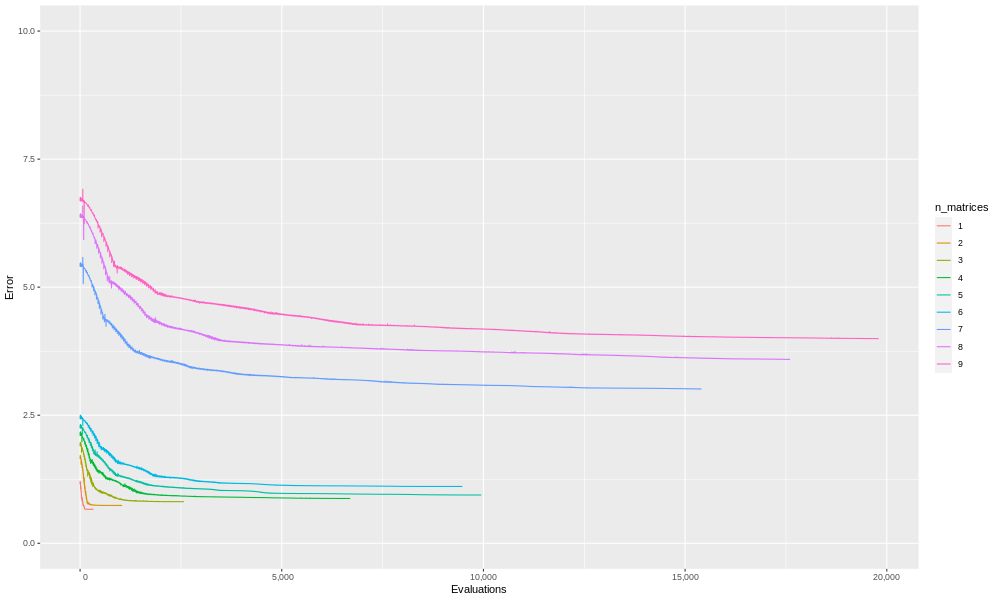
\includegraphics[width=\textwidth]{figures/alg_nelder-mead}
	\decoRule
	\caption[Nelder-Mead]{Nelder-Mead error by iteration step}
	\label{fig:alg_nelder-mead}
\end{figure}

\begin{figure}[!htb]
\centering
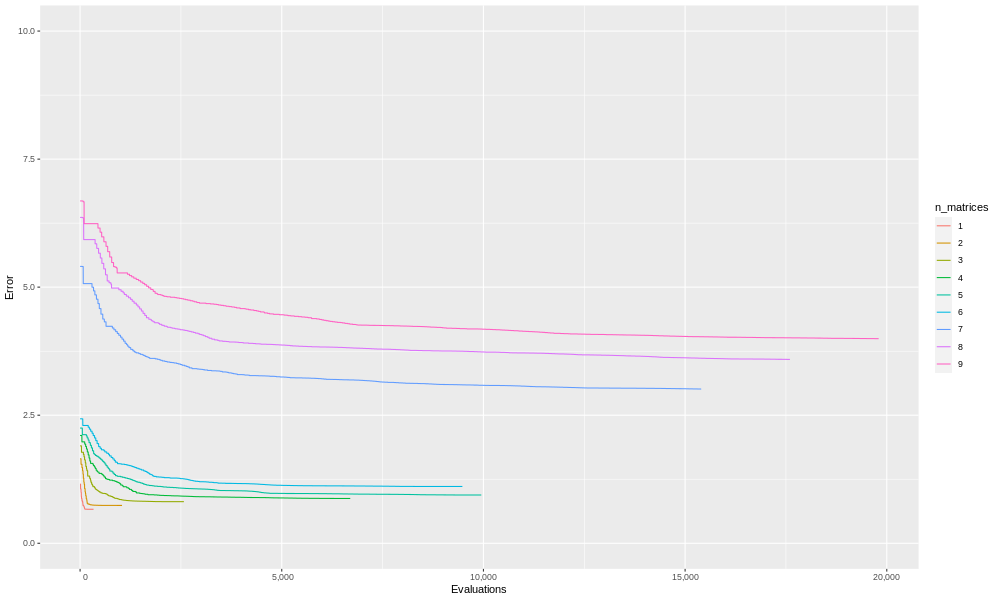
\includegraphics[width=\textwidth]{figures/alg_nelder-mead_smoothed}
\decoRule
\caption[Nelder-Mead (smoothed)]{Nelder-Mead smoothed error by iteration step (cumulative minimum)}
\label{fig:alg_nelder-mead_smoothed}
\end{figure}

\begin{figure}[!htb]
\centering
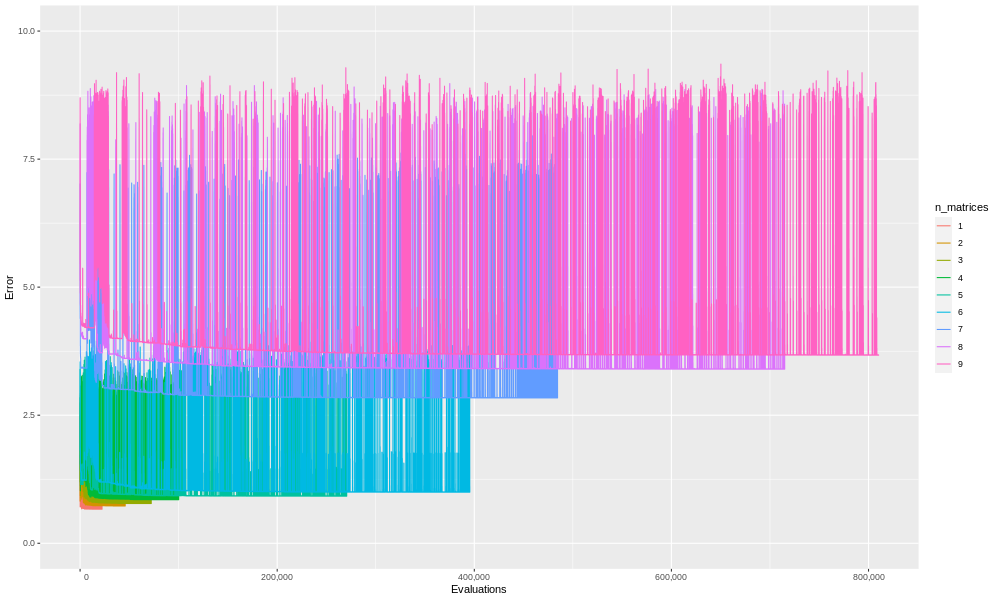
\includegraphics[width=\textwidth]{figures/alg_annealing}
\decoRule
\caption[Simulated Annealing]{Simulated Annealing error by iteration step}
\label{fig:alg_annealing}
\end{figure}

\begin{figure}[!htb]
\centering
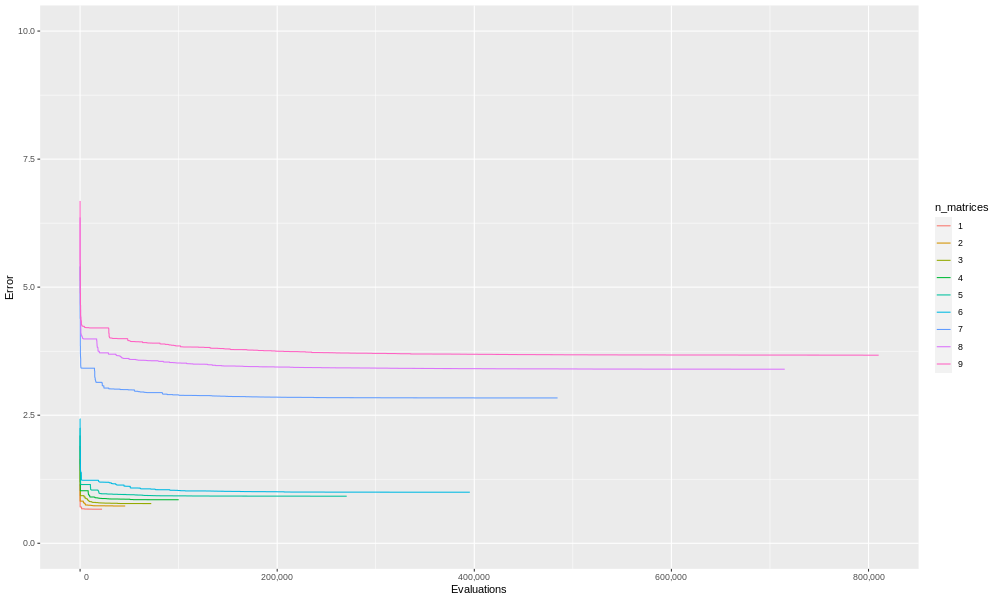
\includegraphics[width=\textwidth]{figures/alg_annealing_smoothed}
\decoRule
\caption[Simulated Annealing (smoothed)]{Simulated Annealing smoothed error by iteration step (cumulative minimum)}
\label{fig:alg_annealing_smoothed}
\end{figure}

\begin{figure}[!htb]
\centering
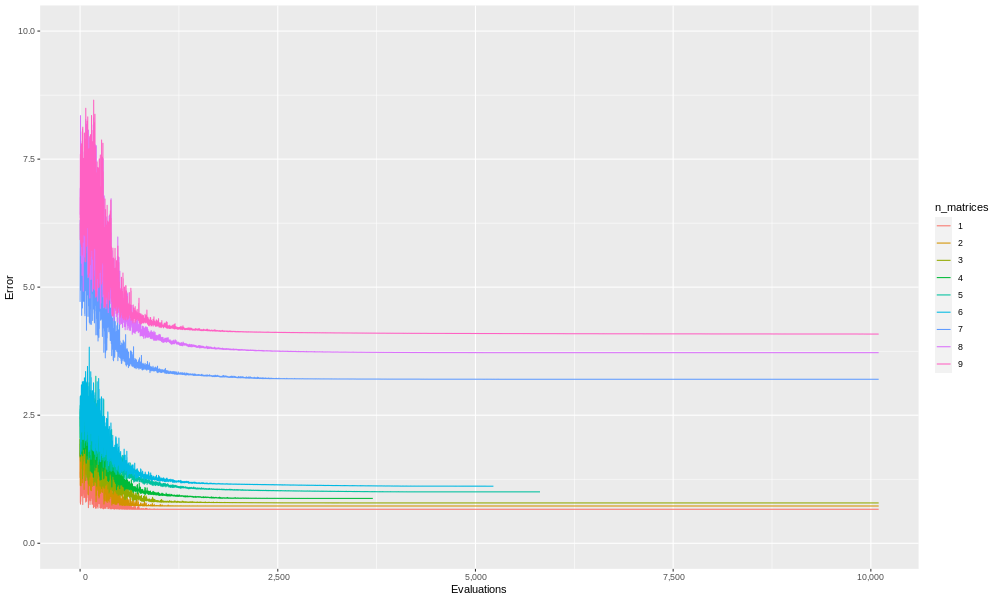
\includegraphics[width=\textwidth]{figures/alg_pso}
\decoRule
\caption[Particle Swarm Optimization]{Particle Swarm Optimization error by iteration step}
\label{fig:alg_pso}
\end{figure}

\begin{figure}[!htb]
\centering
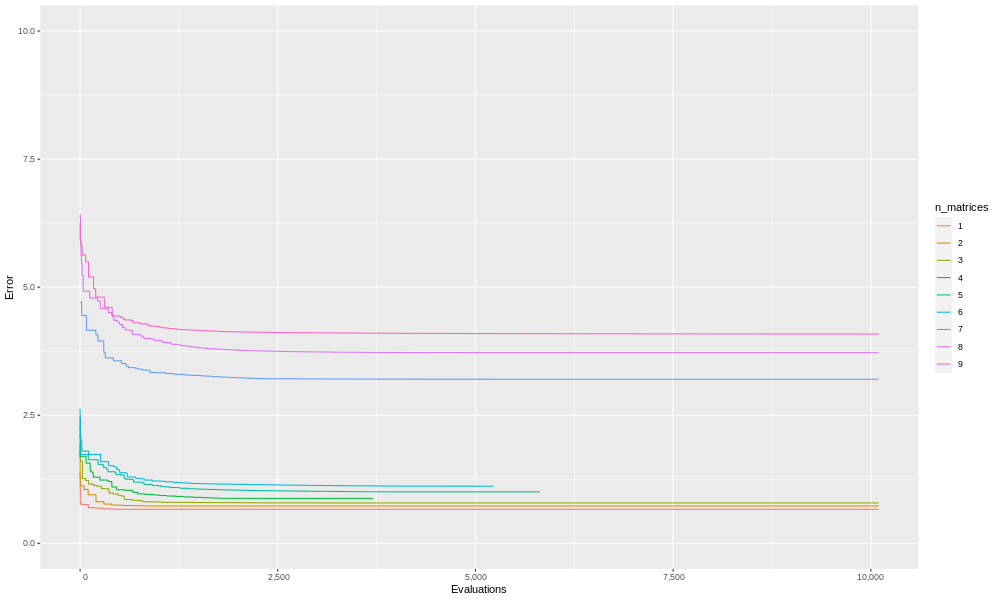
\includegraphics[width=\textwidth]{figures/alg_pso_smoothed}
\decoRule
\caption[Particle Swarm Optimization (smoothed)]{Particle Swarm Optimization smoothed error by iteration step (cumulative minimum)}
\label{fig:alg_pso_smoothed}
\end{figure}

\begin{figure}[!htb]
\centering
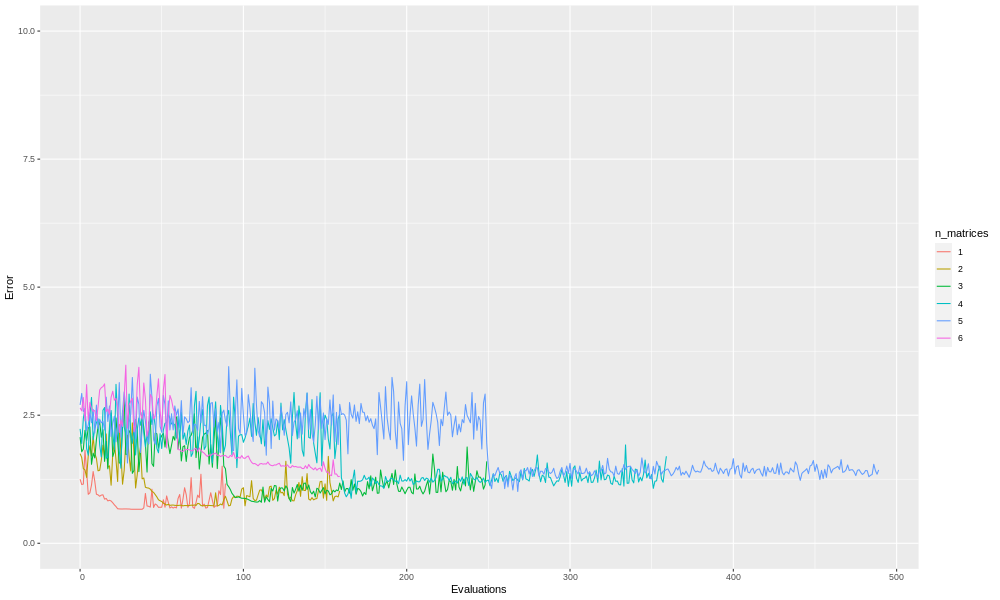
\includegraphics[width=\textwidth]{figures/alg_bayesian}
\decoRule
\caption[Bayesian Optimization]{Bayesian Optimization error by iteration step}
\label{fig:alg_bayesian}
\end{figure}

\begin{figure}[!htb]
\centering
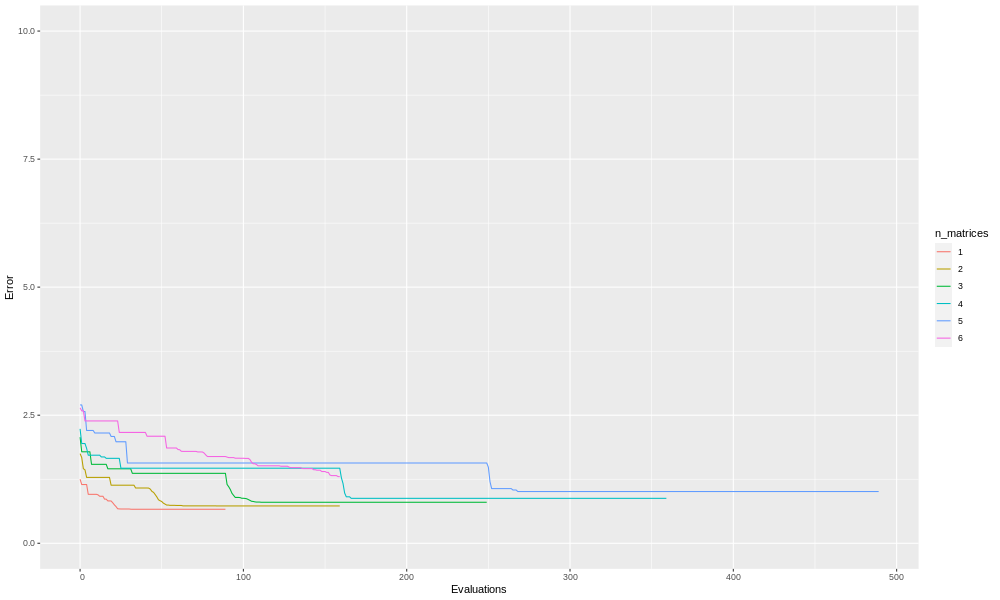
\includegraphics[width=\textwidth]{figures/alg_bayesian_smoothed}
\decoRule
\caption[Bayesian Optimization (smoothed)]{Bayesian Optimization smoothed error by iteration step (cumulative minimum)}
\label{fig:alg_bayesian_smoothed}
\end{figure}


\subsection{Dimensionality comparison}

\begin{figure}[!htb]
	\centering
	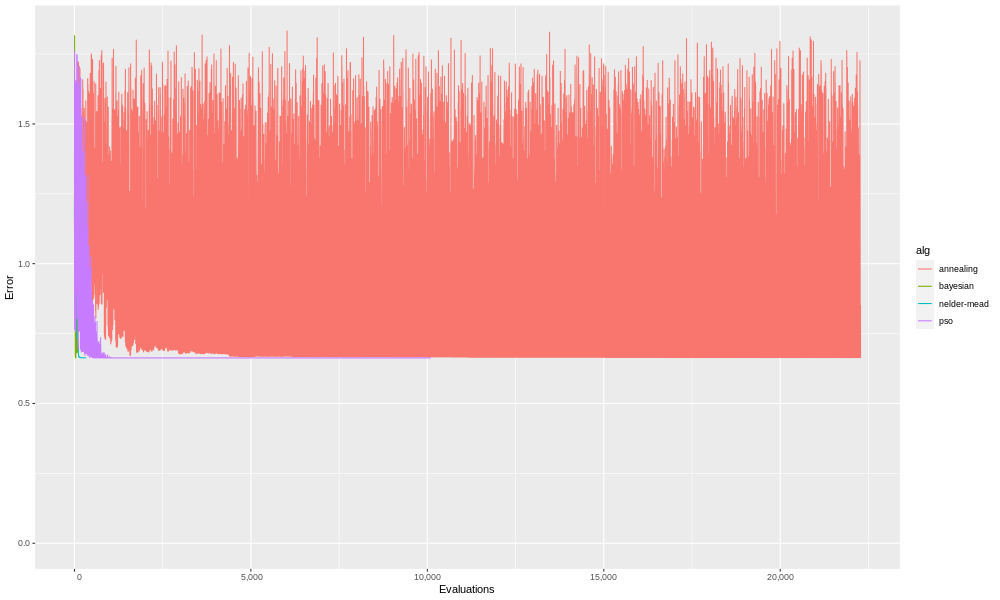
\includegraphics[width=\textwidth]{figures/n_1}
	\decoRule
	\caption[n=1]{Errors on n\_matrices = 1 by method}
	\label{fig:n_1}
\end{figure}

\begin{figure}[!htb]
	\centering
	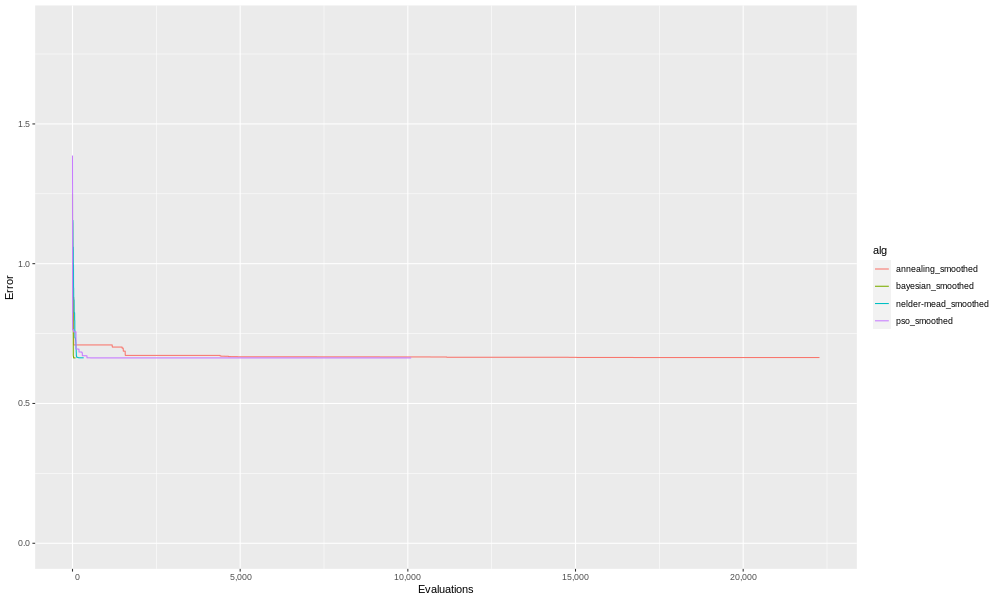
\includegraphics[width=\textwidth]{figures/n_1_smoothed}
	\decoRule
	\caption[n=1 (smoothed)]{(Smoothed) errors on n\_matrices = 1 by method}
	\label{fig:n_1_smoothed}
\end{figure}

\begin{figure}[!htb]
\centering
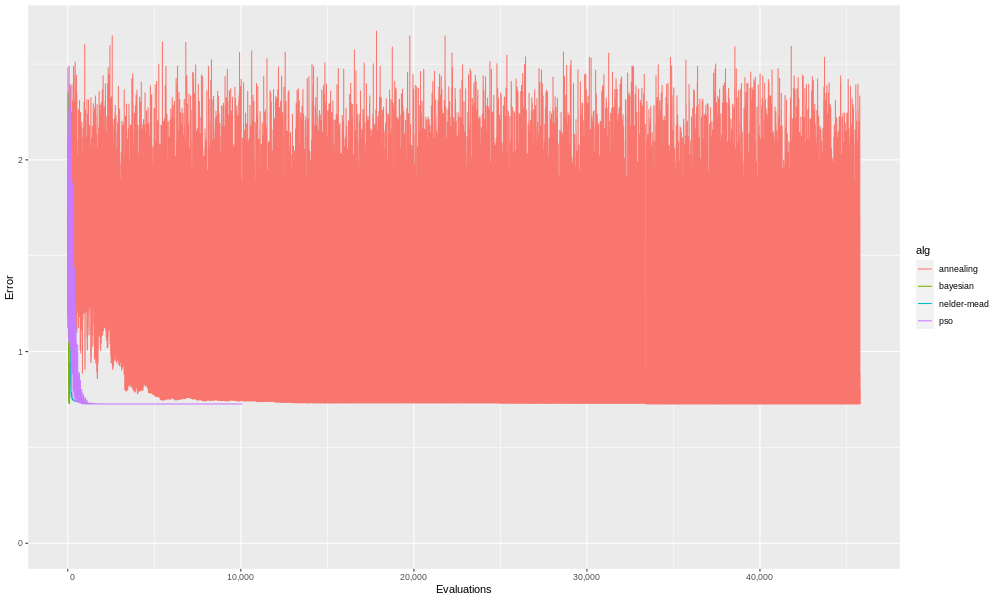
\includegraphics[width=\textwidth]{figures/n_2}
\decoRule
\caption[n=2]{Errors on n\_matrices = 2 by method}
\label{fig:n_2}
\end{figure}

\begin{figure}[!htb]
\centering
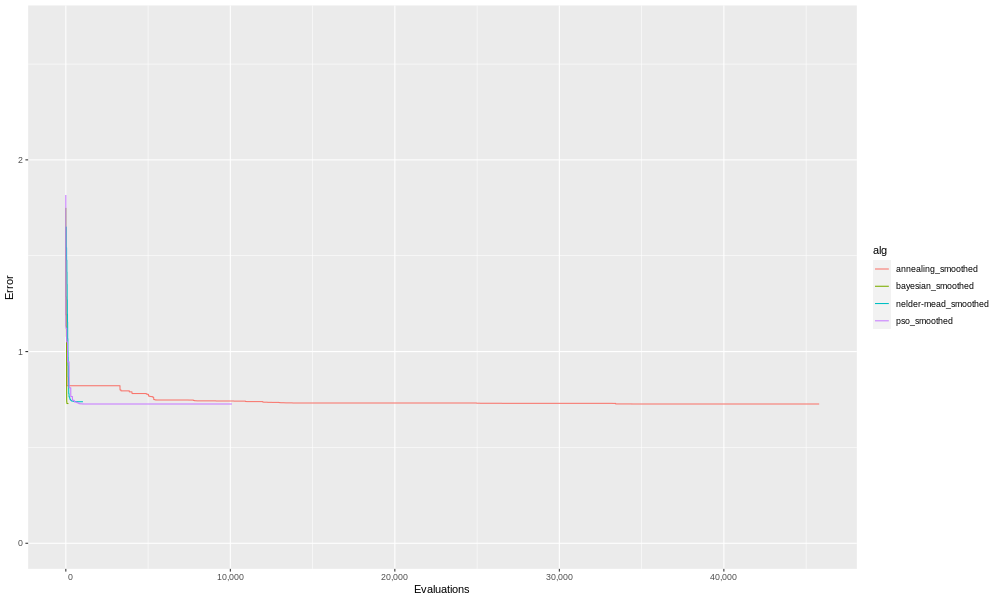
\includegraphics[width=\textwidth]{figures/n_2_smoothed}
\decoRule
\caption[n=2 (smoothed)]{(Smoothed) errors on n\_matrices = 2 by method}
\label{fig:n_2_smoothed}
\end{figure}

\begin{figure}[!htb]
\centering
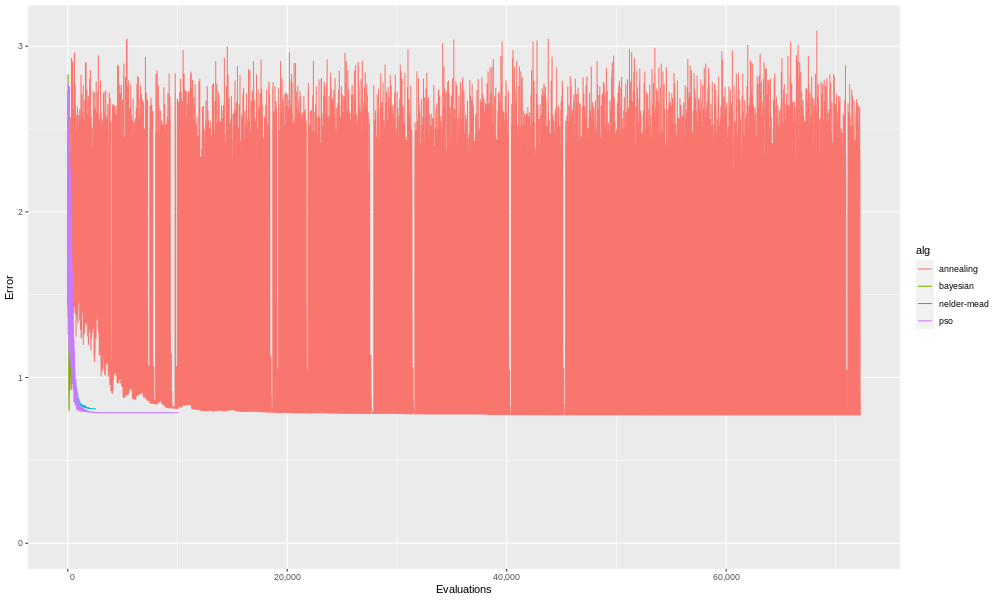
\includegraphics[width=\textwidth]{figures/n_3}
\decoRule
\caption[n=3]{Errors on n\_matrices = 3 by method}
\label{fig:n_3}
\end{figure}

\begin{figure}[!htb]
\centering
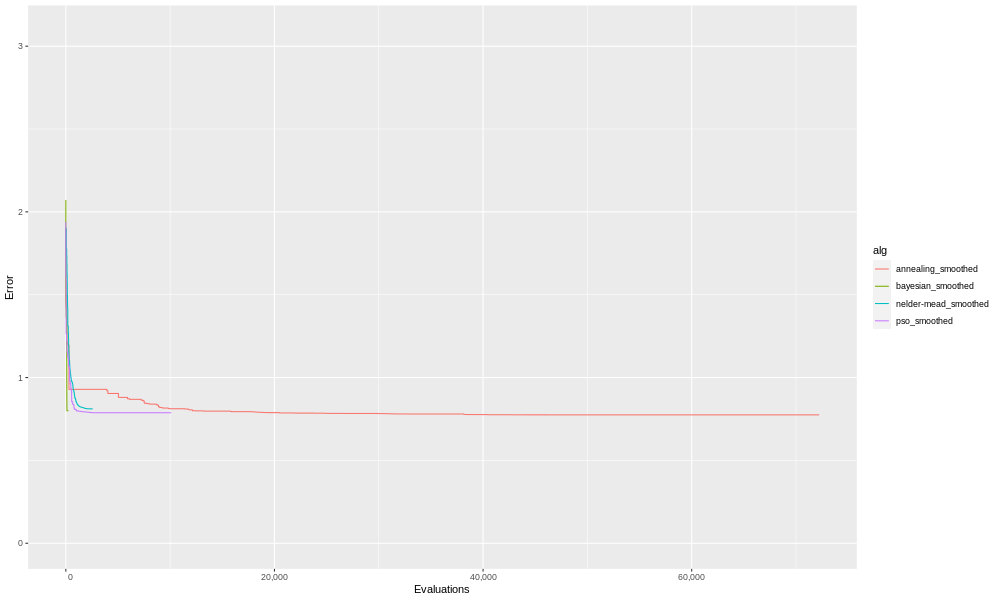
\includegraphics[width=\textwidth]{figures/n_3_smoothed}
\decoRule
\caption[n=3 (smoothed)]{(Smoothed) errors on n\_matrices = 3 by method}
\label{fig:n_3_smoothed}
\end{figure}

\begin{figure}[!htb]
\centering
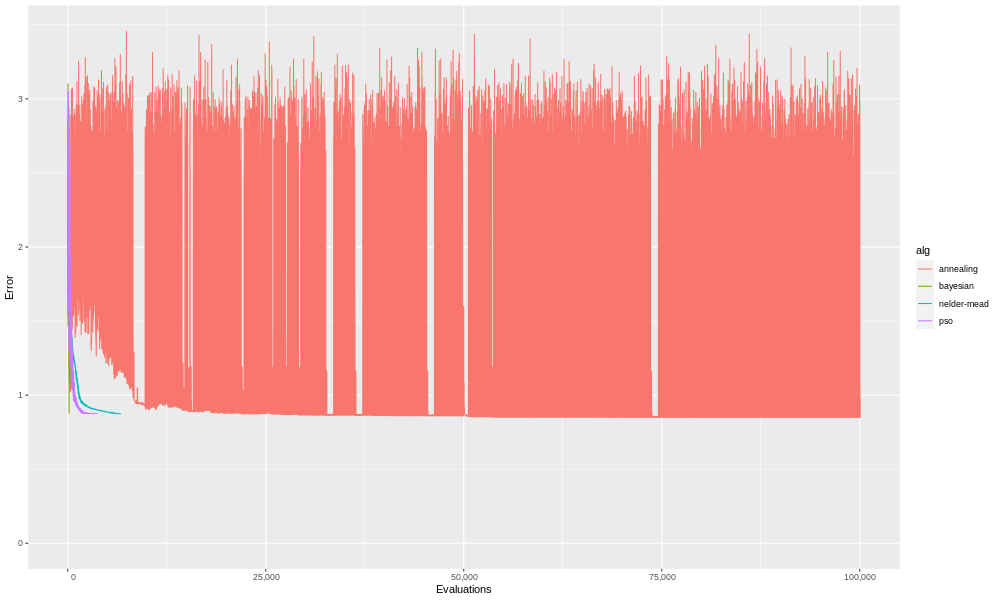
\includegraphics[width=\textwidth]{figures/n_4}
\decoRule
\caption[n=4]{Errors on n\_matrices = 4 by method}
\label{fig:n_4}
\end{figure}

\begin{figure}[!htb]
\centering
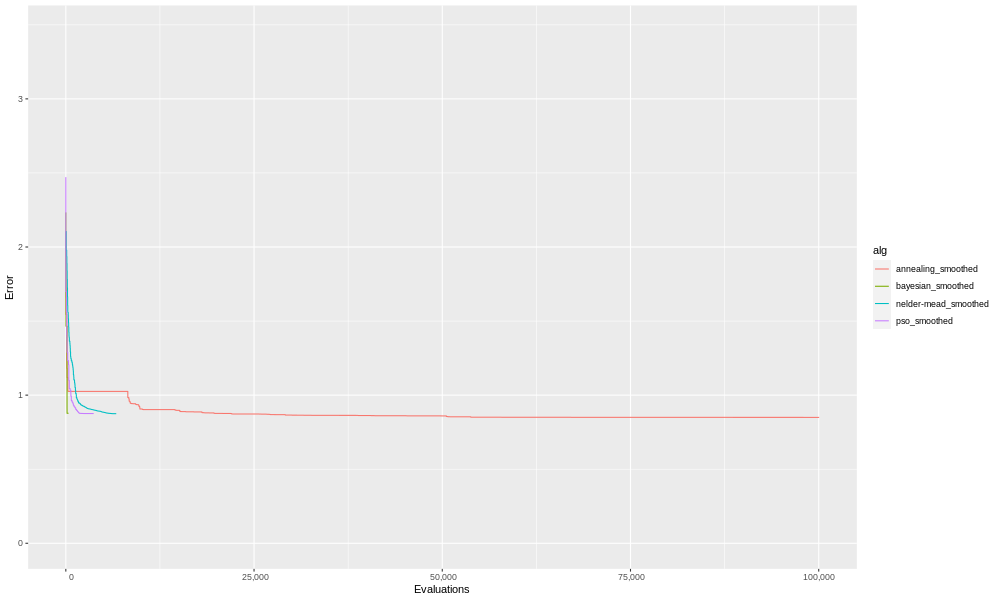
\includegraphics[width=\textwidth]{figures/n_4_smoothed}
\decoRule
\caption[n=4 (smoothed)]{(Smoothed) errors on n\_matrices = 4 by method}
\label{fig:n_4_smoothed}
\end{figure}

\begin{figure}[!htb]
\centering
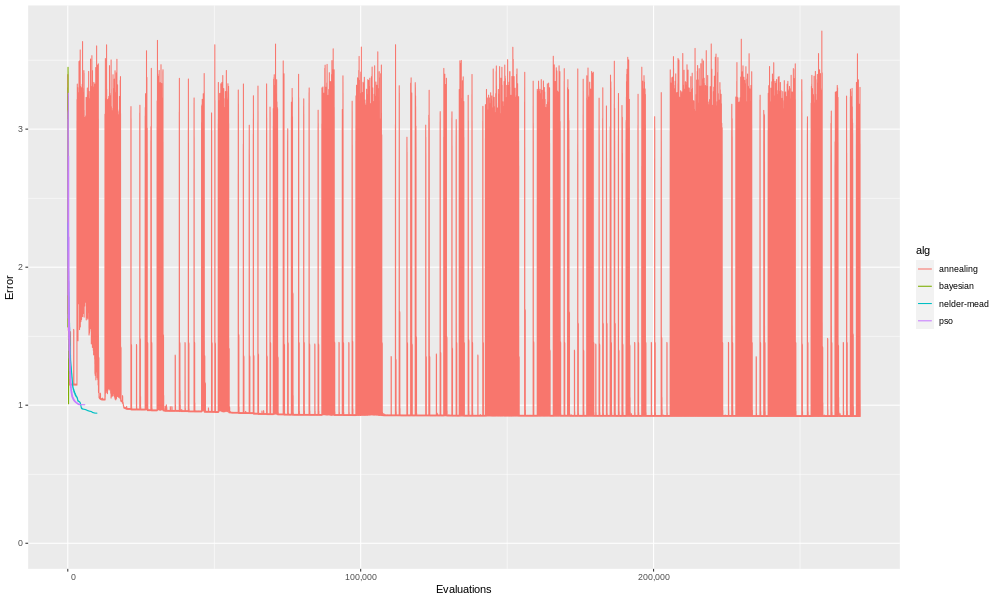
\includegraphics[width=\textwidth]{figures/n_5}
\decoRule
\caption[n=5]{Errors on n\_matrices = 5 by method}
\label{fig:n_5}
\end{figure}

\begin{figure}[!htb]
\centering
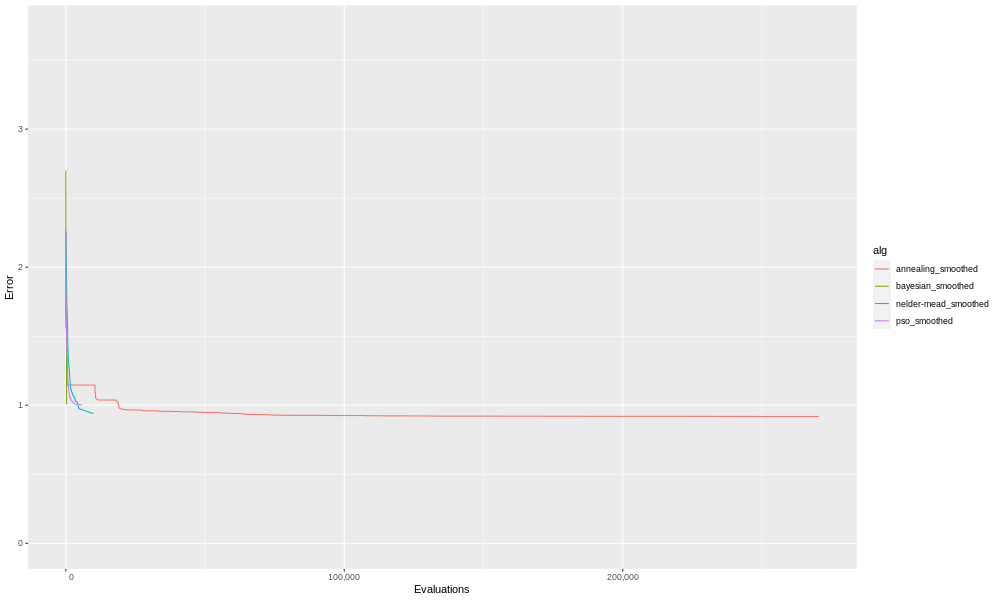
\includegraphics[width=\textwidth]{figures/n_5_smoothed}
\decoRule
\caption[n=5 (smoothed)]{(Smoothed) errors on n\_matrices = 5 by method}
\label{fig:n_5_smoothed}
\end{figure}

\begin{figure}[!htb]
\centering
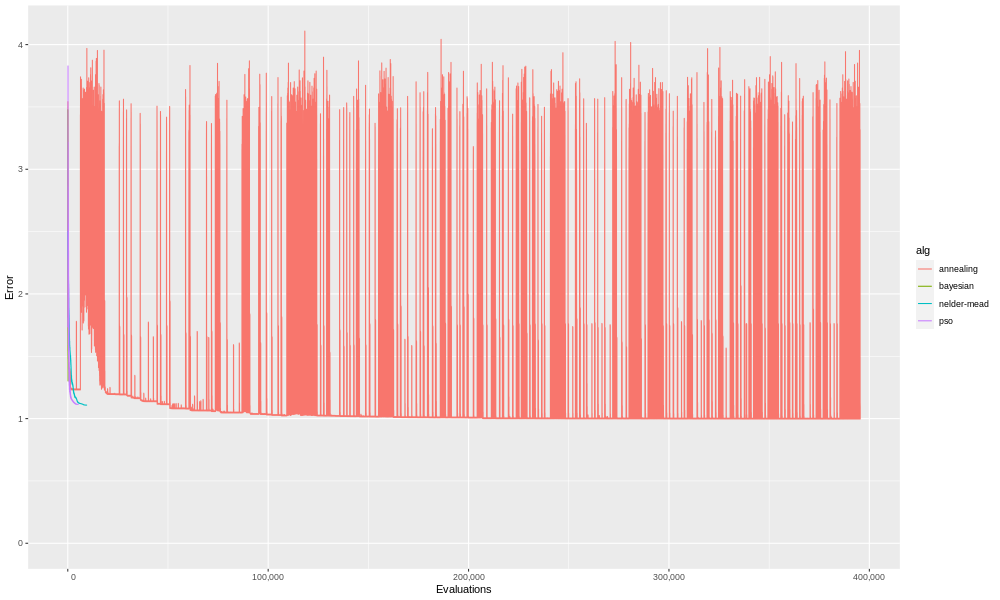
\includegraphics[width=\textwidth]{figures/n_6}
\decoRule
\caption[n=6]{Errors on n\_matrices = 6 by method}
\label{fig:n_6}
\end{figure}

\begin{figure}[!htb]
\centering
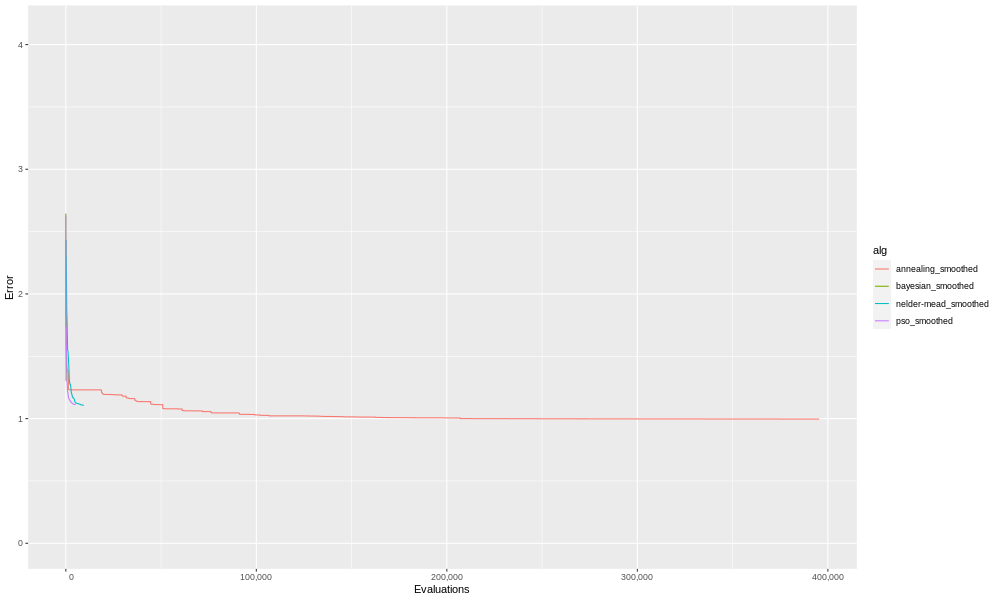
\includegraphics[width=\textwidth]{figures/n_6_smoothed}
\decoRule
\caption[n=6 (smoothed)]{(Smoothed) errors on n\_matrices = 6 by method}
\label{fig:n_6_smoothed}
\end{figure}

\begin{figure}[!htb]
\centering
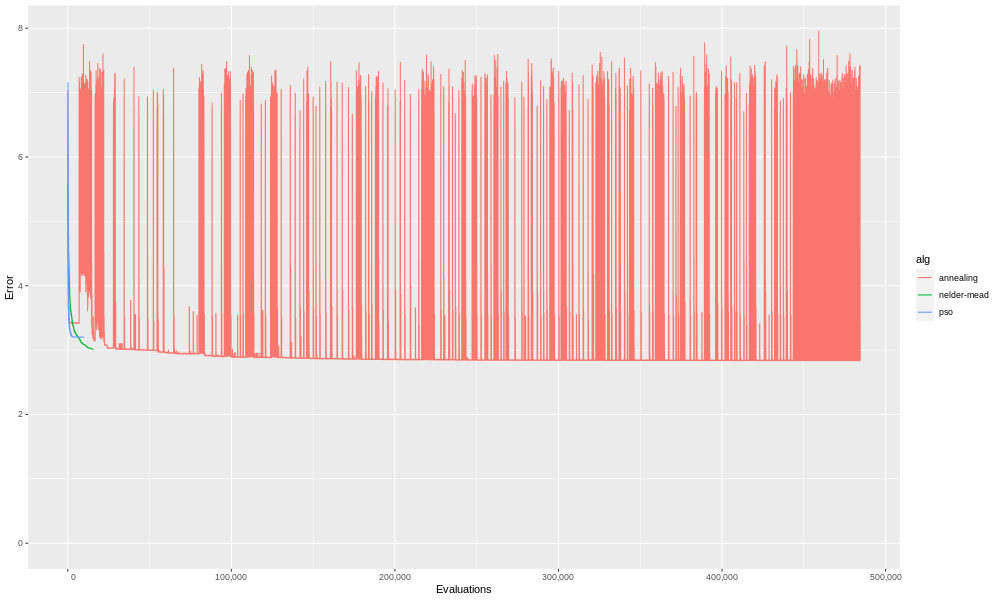
\includegraphics[width=\textwidth]{figures/n_7}
\decoRule
\caption[n=7]{Errors on n\_matrices = 7 by method}
\label{fig:n_7}
\end{figure}

\begin{figure}[!htb]
\centering
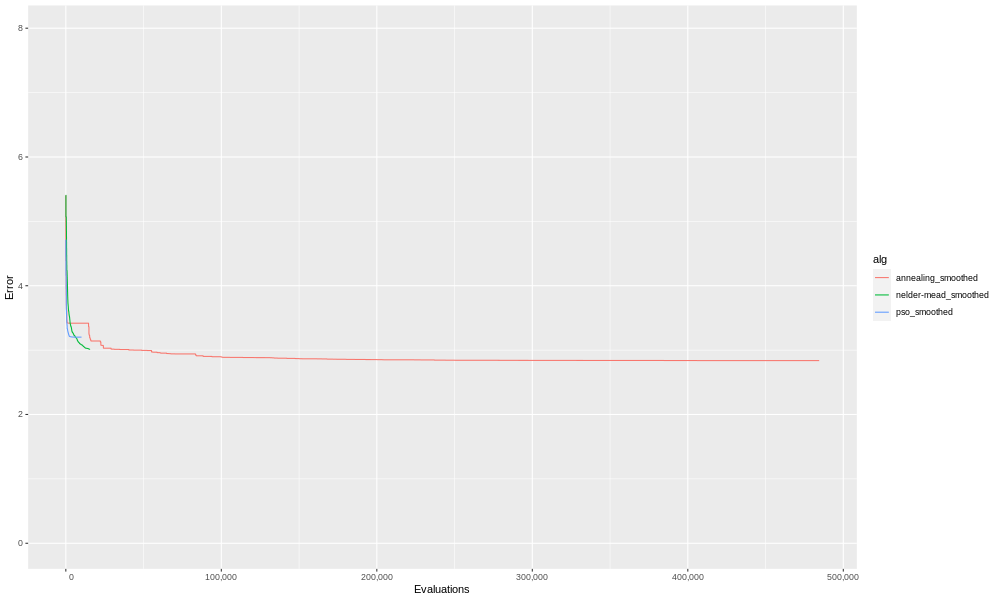
\includegraphics[width=\textwidth]{figures/n_7_smoothed}
\decoRule
\caption[n=7 (smoothed)]{(Smoothed) errors on n\_matrices = 7 by method}
\label{fig:n_7_smoothed}
\end{figure}

\begin{figure}[!htb]
\centering
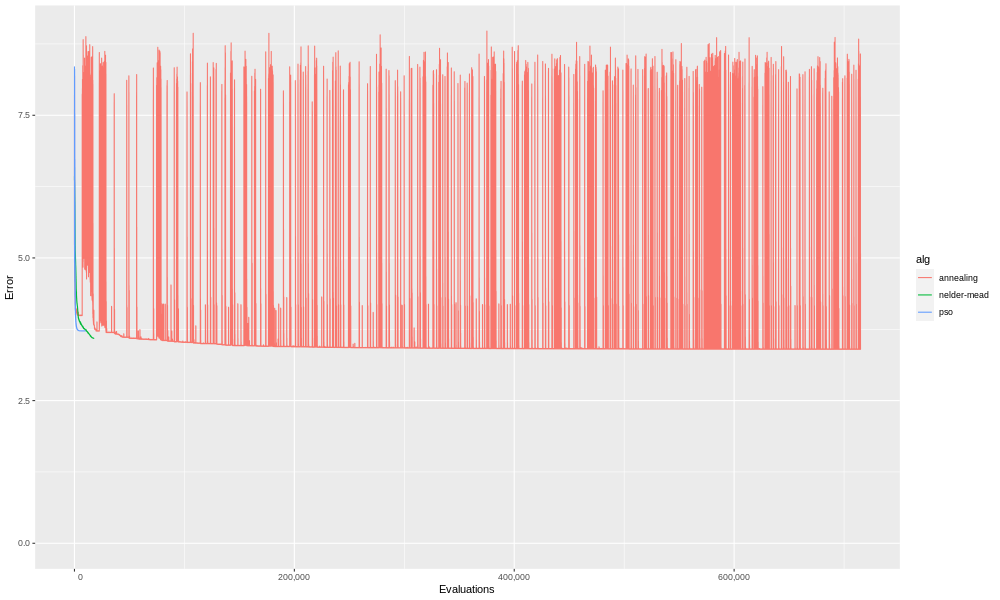
\includegraphics[width=\textwidth]{figures/n_8}
\decoRule
\caption[n=8]{Errors on n\_matrices = 8 by method}
\label{fig:n_8}
\end{figure}

\begin{figure}[!htb]
\centering
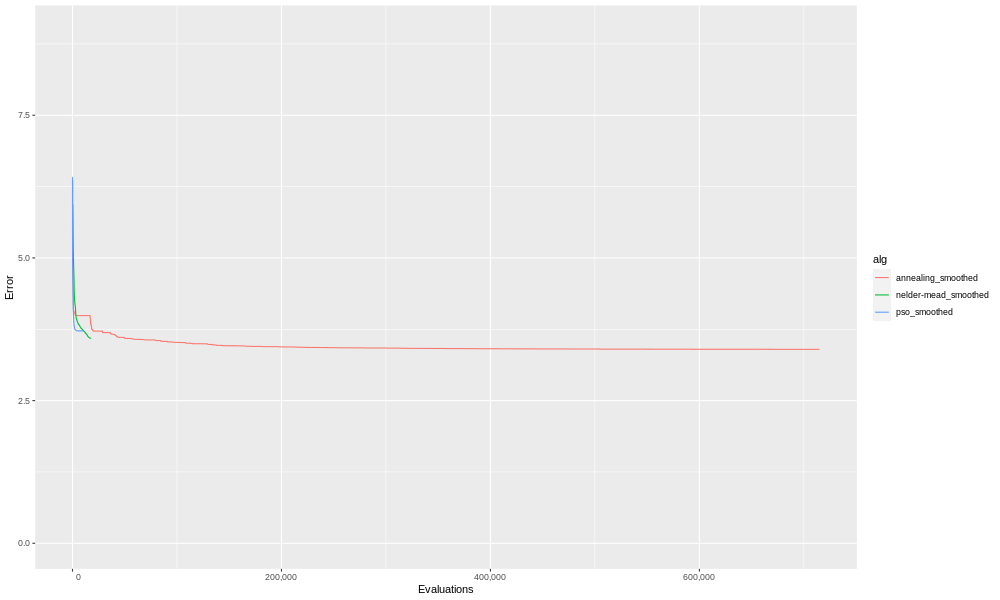
\includegraphics[width=\textwidth]{figures/n_8_smoothed}
\decoRule
\caption[n=8 (smoothed)]{(Smoothed) errors on n\_matrices = 8 by method}
\label{fig:n_8_smoothed}
\end{figure}

\begin{figure}[!htb]
\centering
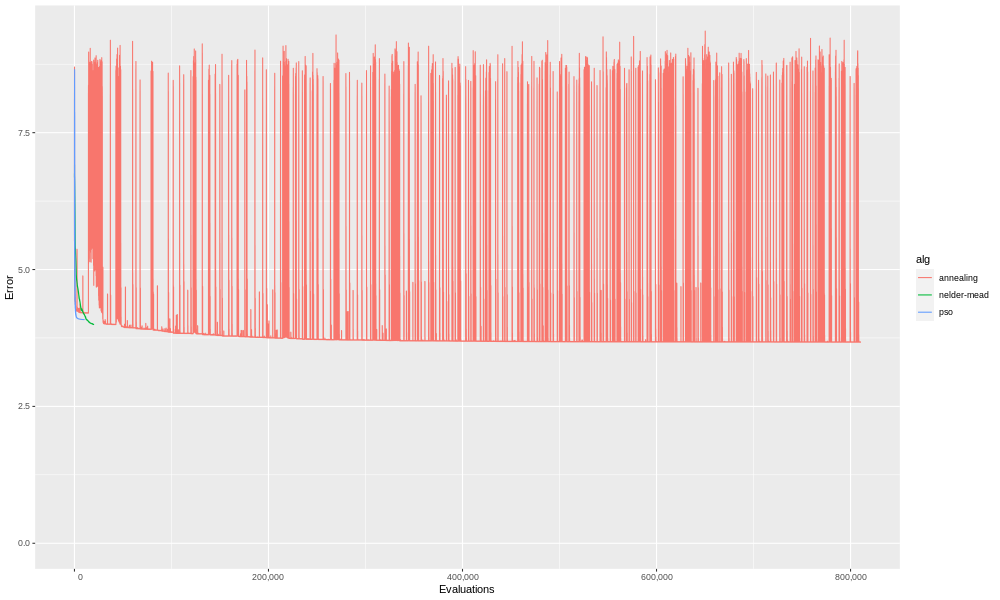
\includegraphics[width=\textwidth]{figures/n_9}
\decoRule
\caption[n=9]{Errors on n\_matrices = 9 by method}
\label{fig:n_9}
\end{figure}

\begin{figure}[!htb]
\centering
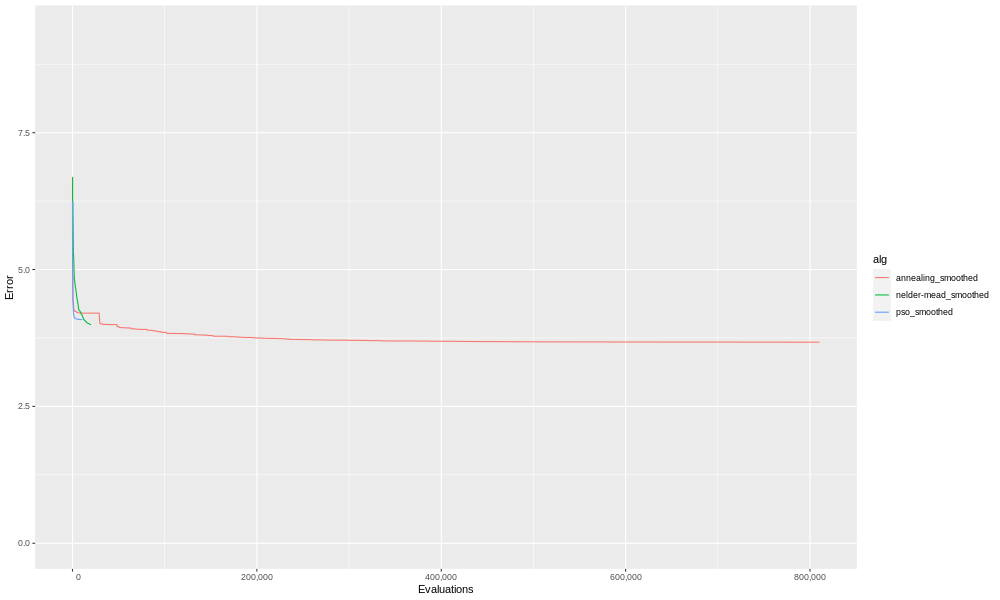
\includegraphics[width=\textwidth]{figures/n_9_smoothed}
\decoRule
\caption[n=9 (smoothed)]{(Smoothed) errors on n\_matrices = 9 by method}
\label{fig:n_9_smoothed}
\end{figure}



\section{Bayesian Optimization (BO) tests}

\begin{figure}[h!]
	\centering
	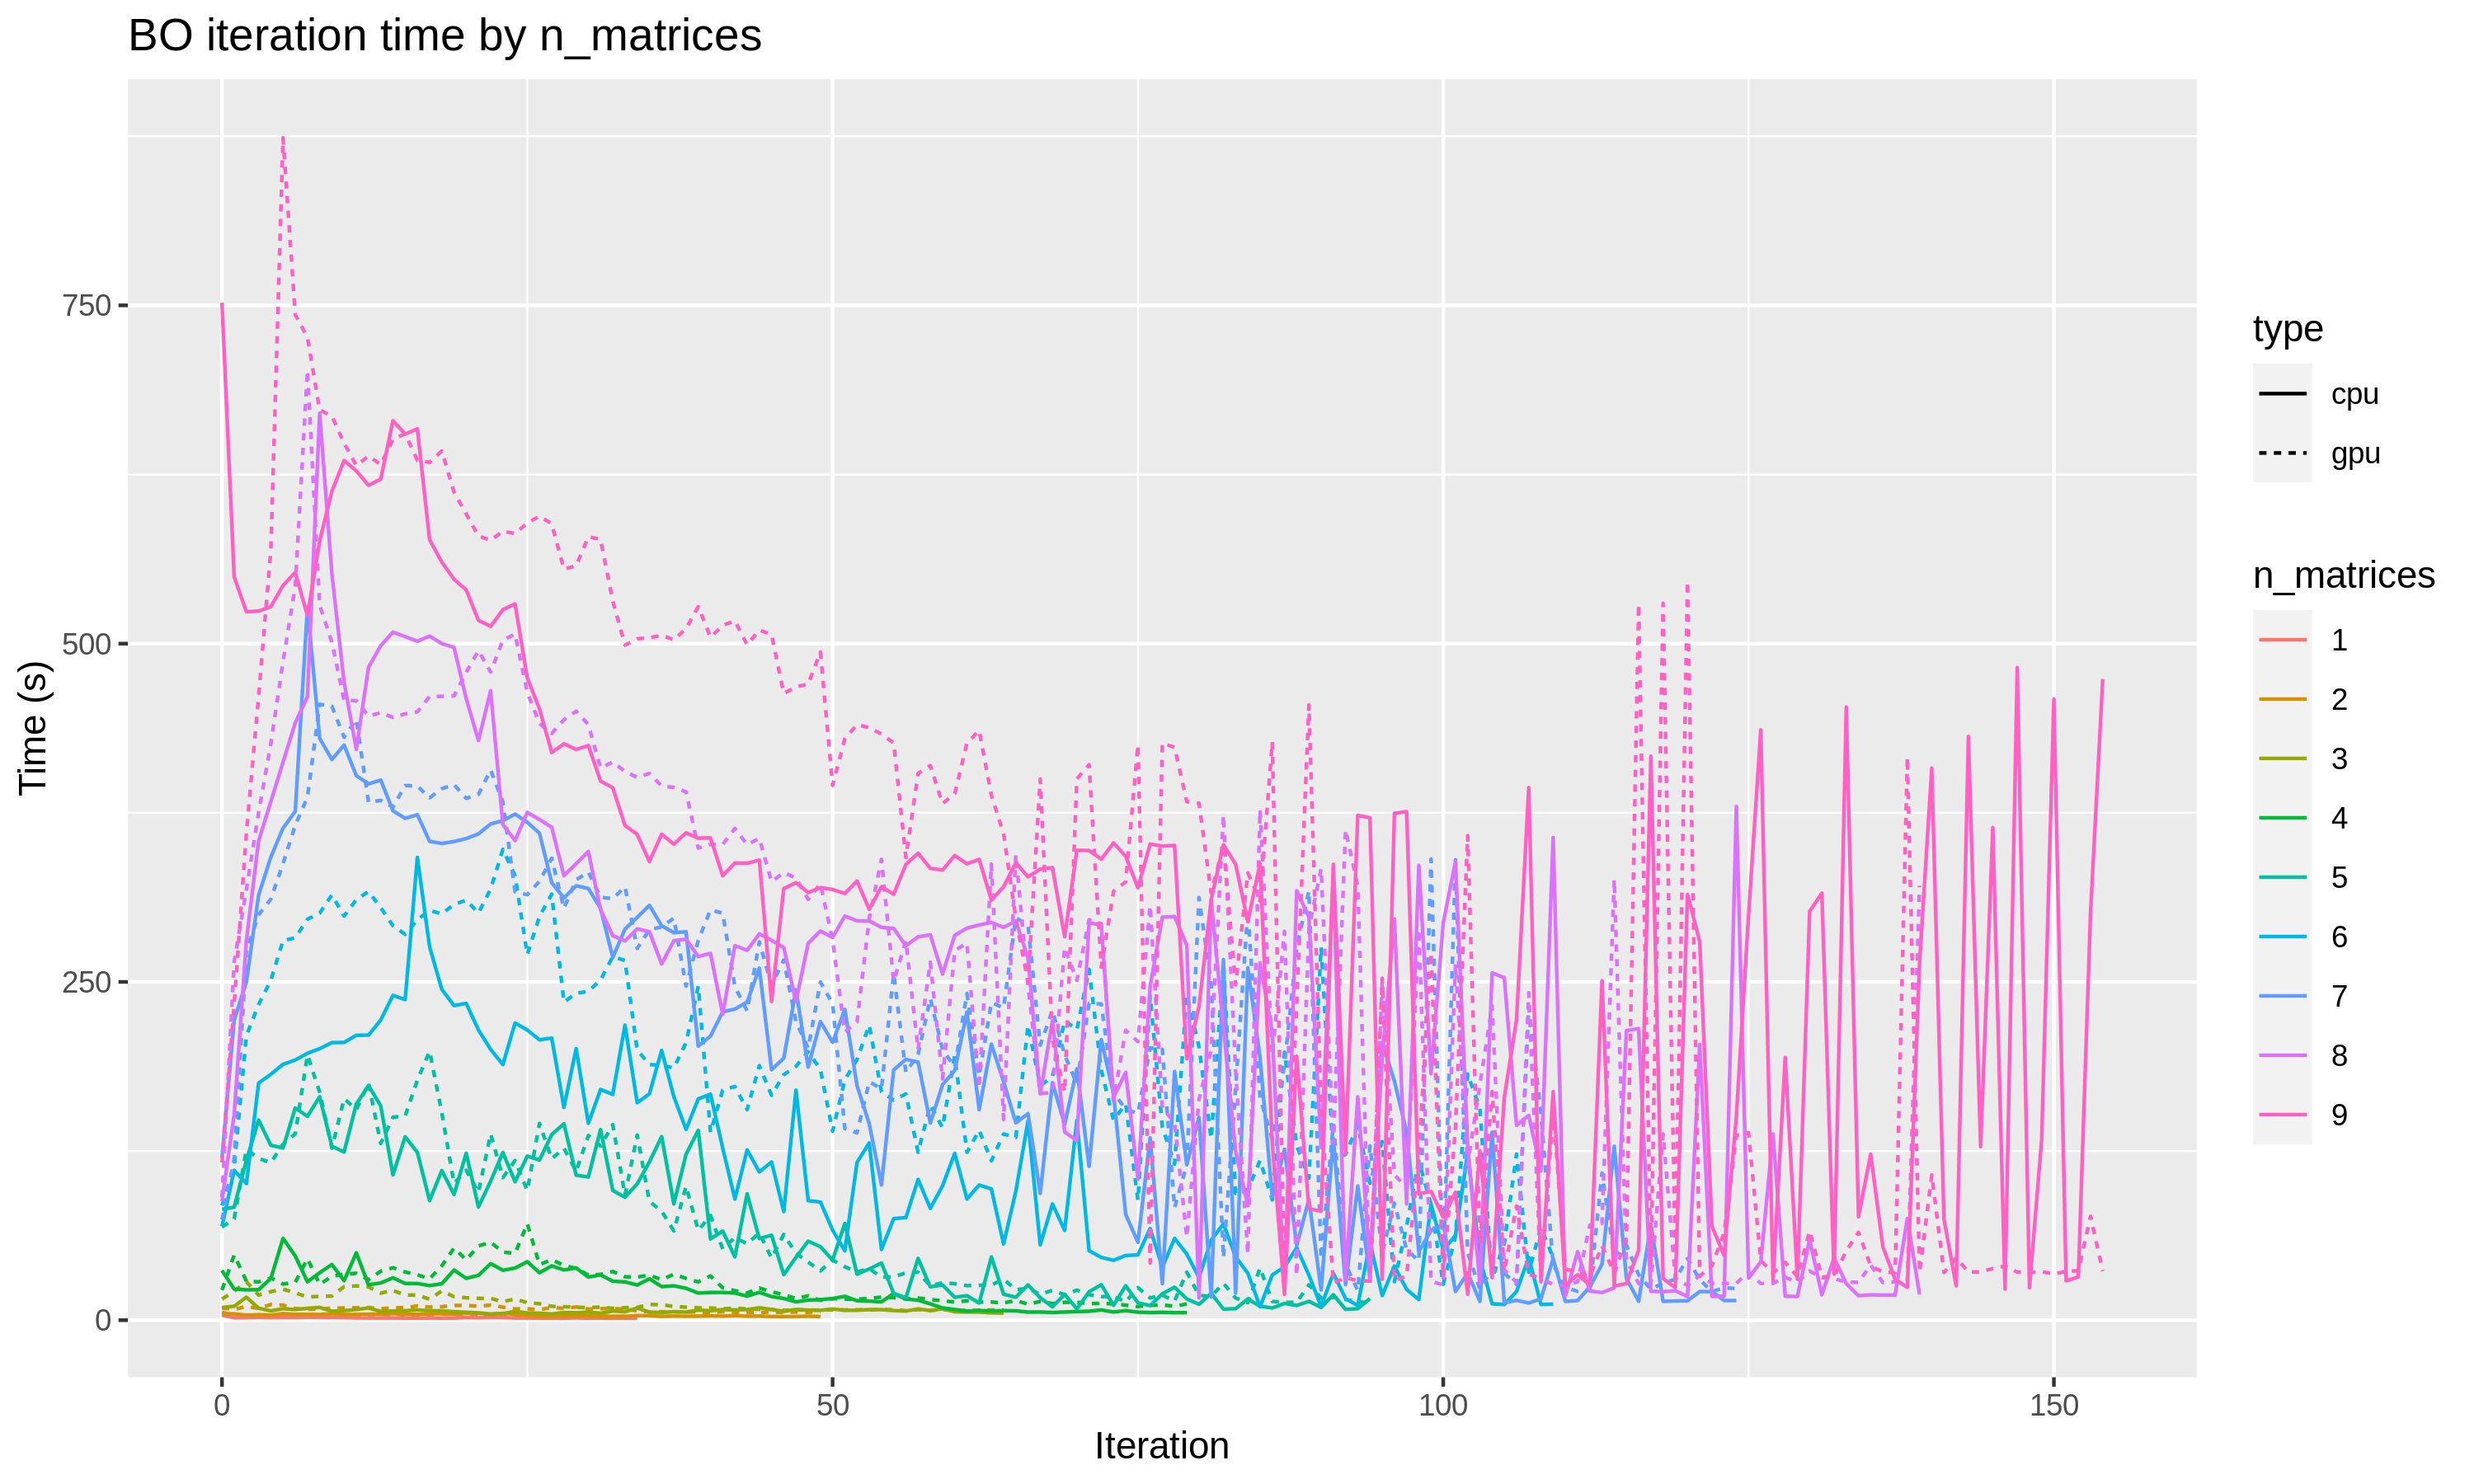
\includegraphics[width=\textwidth]{figures/bo_time}
	\decoRule
	\caption[BO iteration time]{BO iteration time. It increases when the dimensionality increases (different colors) but surprisingly the first iterations take more time than the latter ones, where the opposite is expected. This is a transitory effect as can be seen in figure \ref{fig:bo_time_cpu_long}, using a larger number of iterations. Another surprising outcome is the GPU computation (using a NVIDIA Quadro P620) takes more time than the CPU, but figure \ref{fig:bo_boxplot} shows that the differences are not likely to be significant in the long run. With a powerful GPU this result is expected to change.}
	\label{fig:bo_time}
\end{figure}

\begin{figure}[h!]
\centering
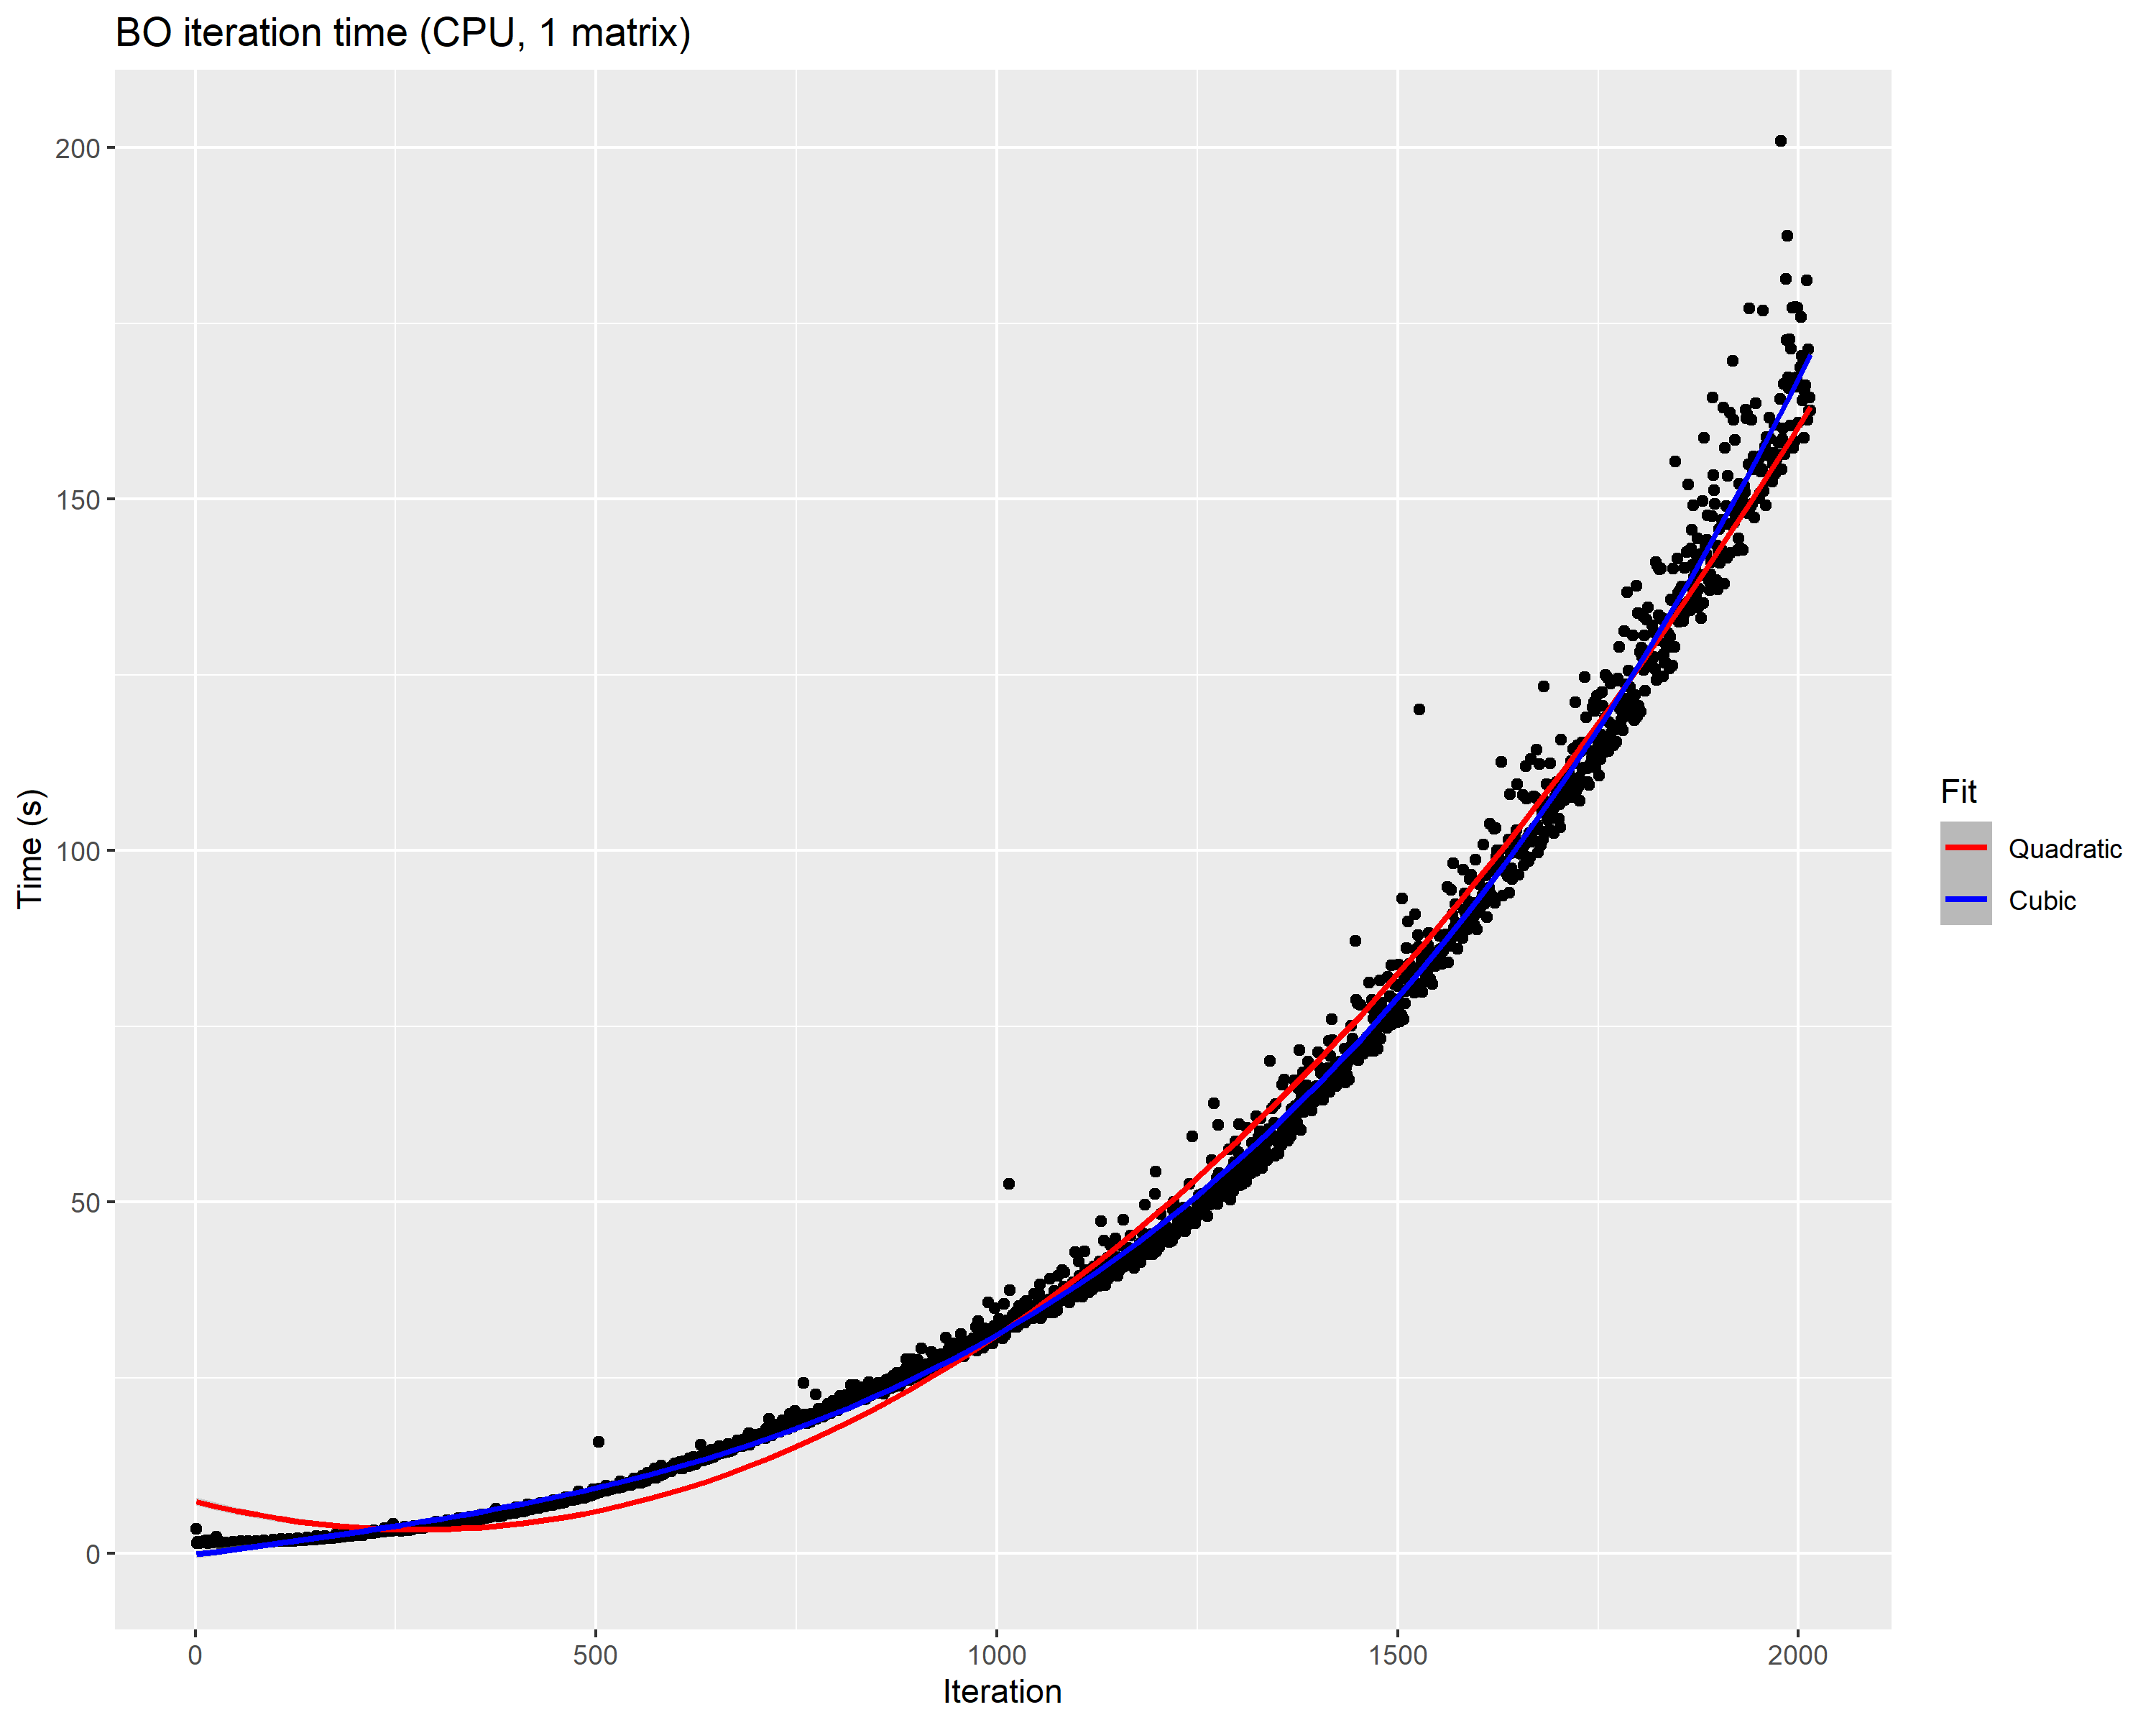
\includegraphics[width=\textwidth]{figures/bo_time_cpu_long}
\decoRule
\caption[CPU BO iteration time (2)]{CPU BO iteration time using a larger number of iterations. It is clear that the iteration times follow a cubic polynomial trend, due to the matrix inversion required in the gaussian process regression stage of the optimization procedure, as seen in figure \ref{fig:gaussian_process_regression}.}
\label{fig:bo_time_cpu_long}
\end{figure}

\begin{figure}[h!]
\centering
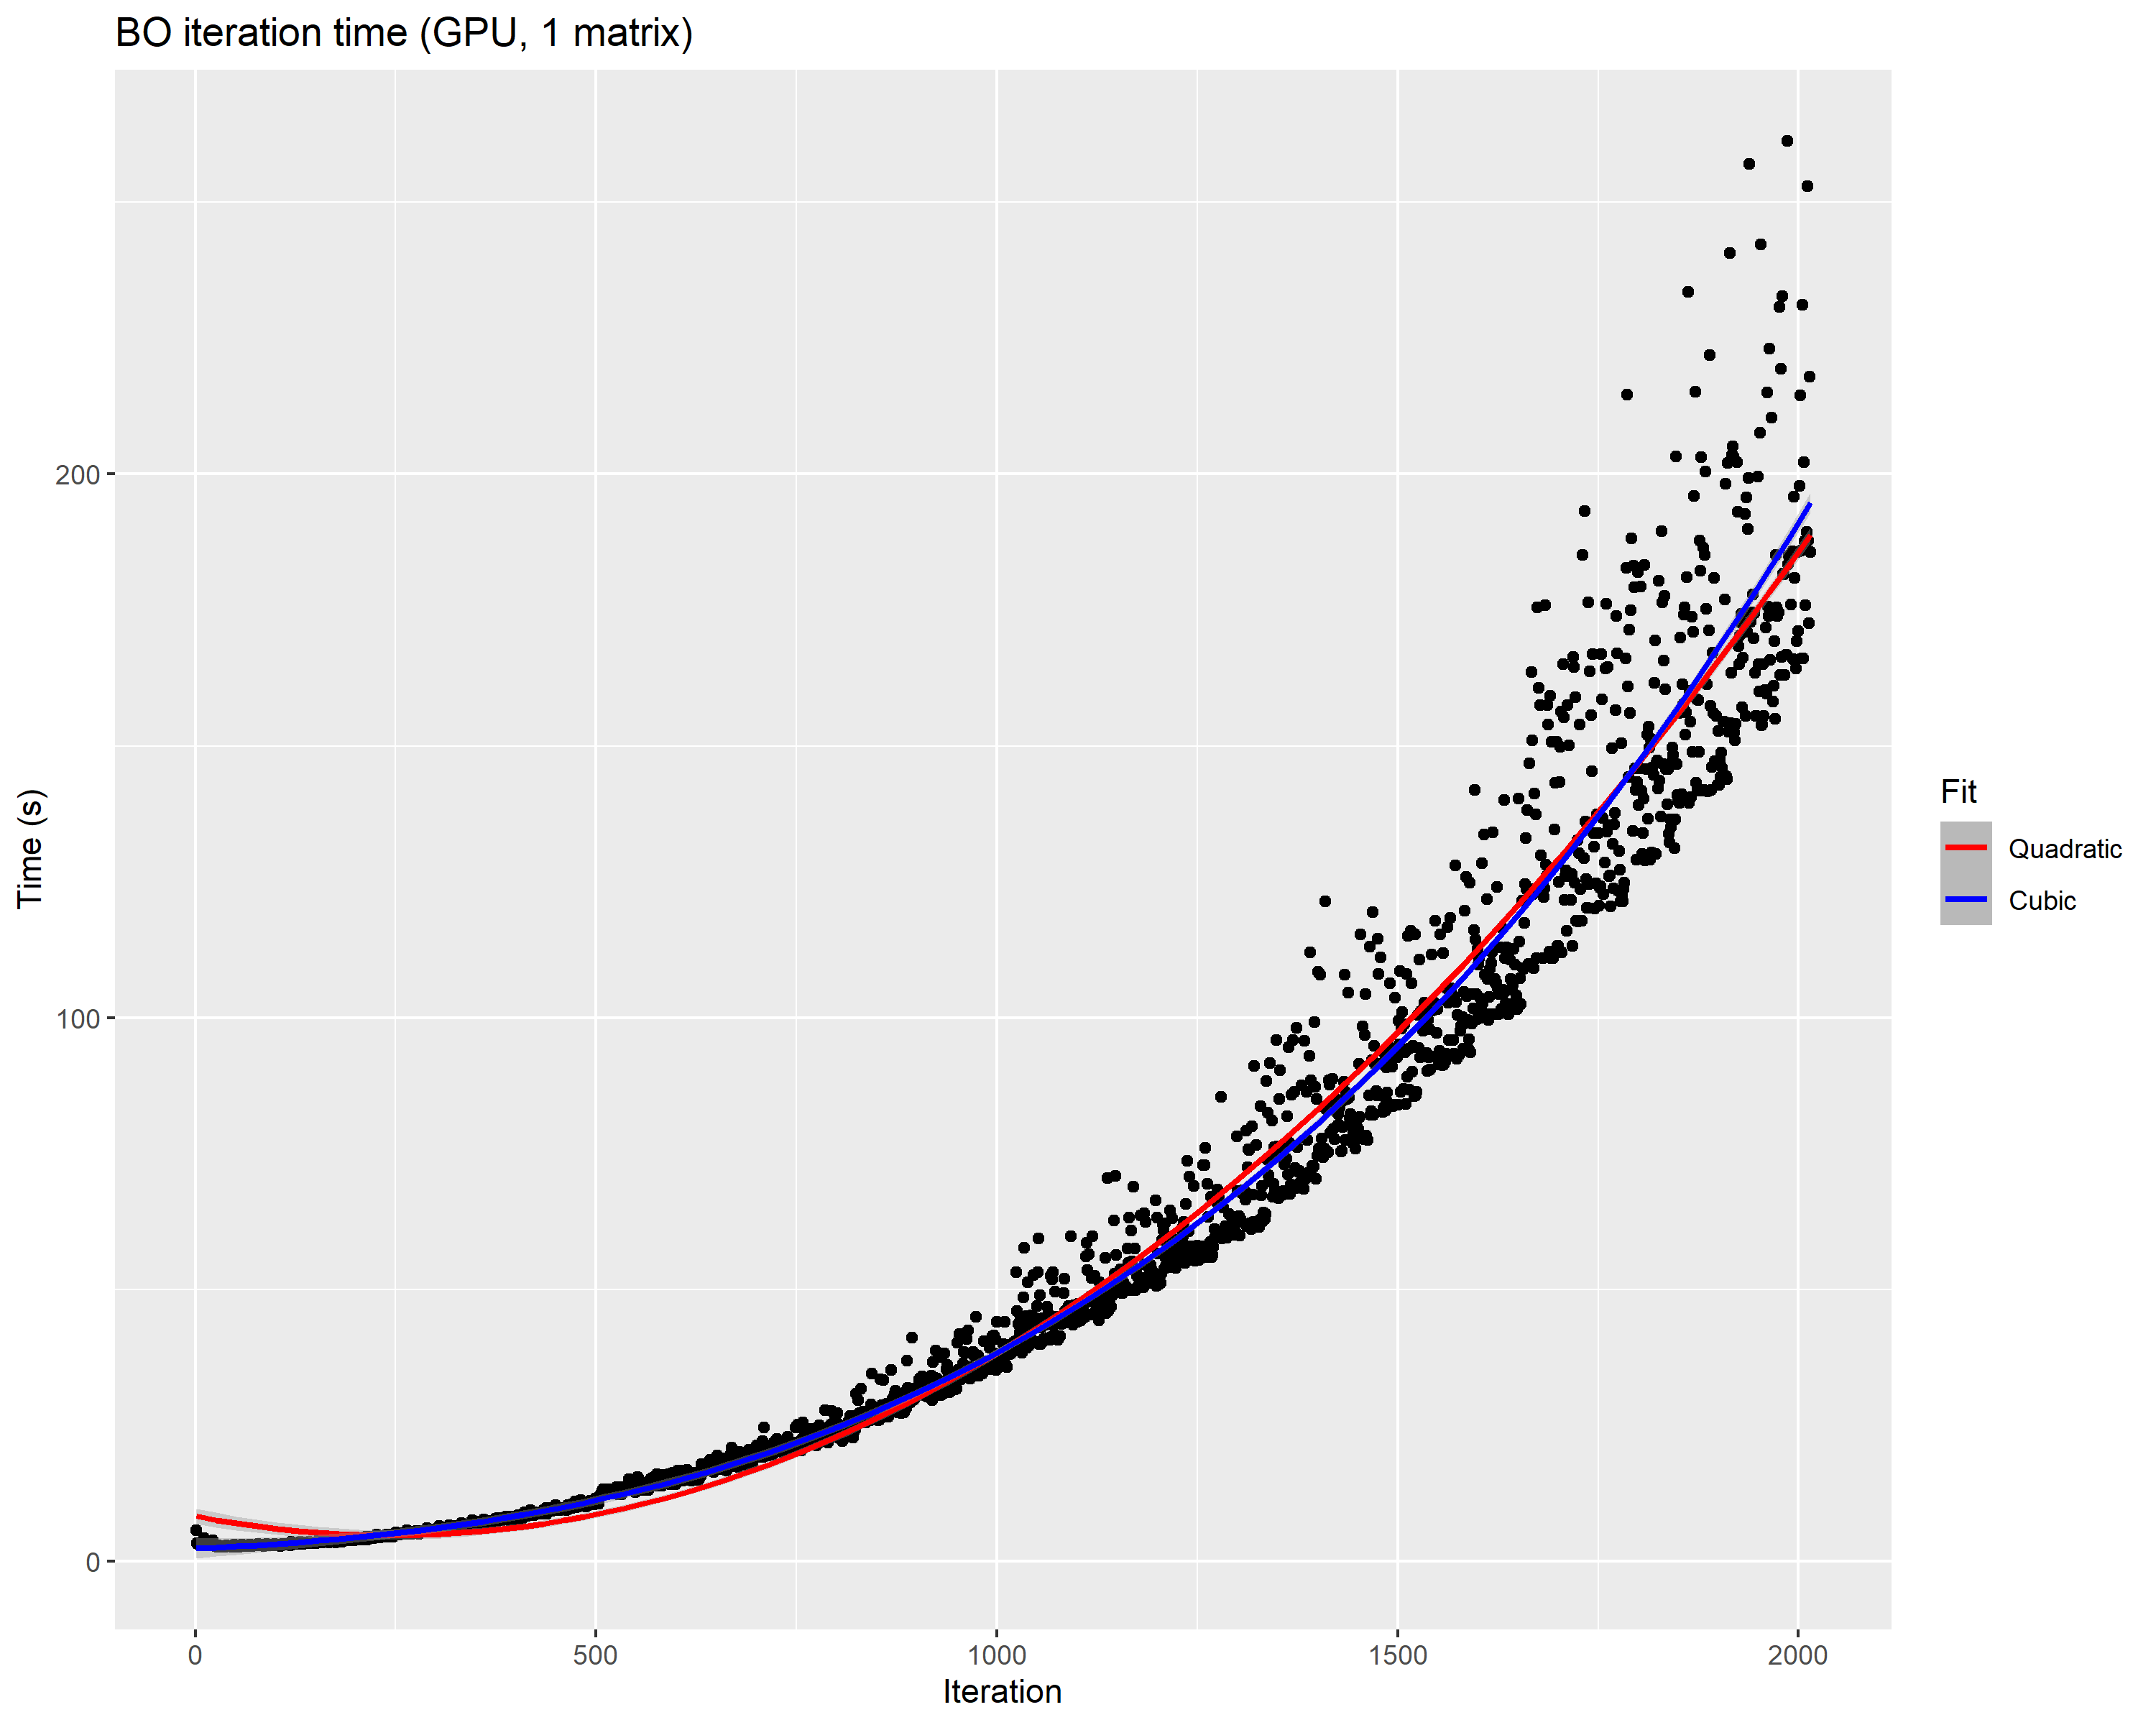
\includegraphics[width=\textwidth]{figures/bo_time_gpu_long}
\decoRule
\caption[GPU BO iteration time (2)]{GPU BO iteration time using a larger number of iterations. It is clear as well that the iteration times follow a cubic polynomial trend as the CPU optimization, but with a larger variance in the last iterations.}
\label{fig:bo_time_gpu_long}
\end{figure}

\begin{figure}[h!]
\centering
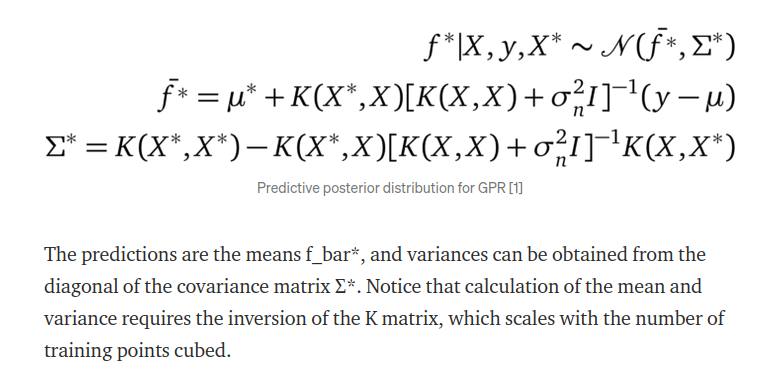
\includegraphics[width=\textwidth]{figures/gaussian_process_regression}
\decoRule
\caption[Gaussian process predictive posterior distribution]{Gaussian process predictive posterior distribution}
\label{fig:gaussian_process_regression}
\end{figure}

\begin{figure}[h!]
\centering
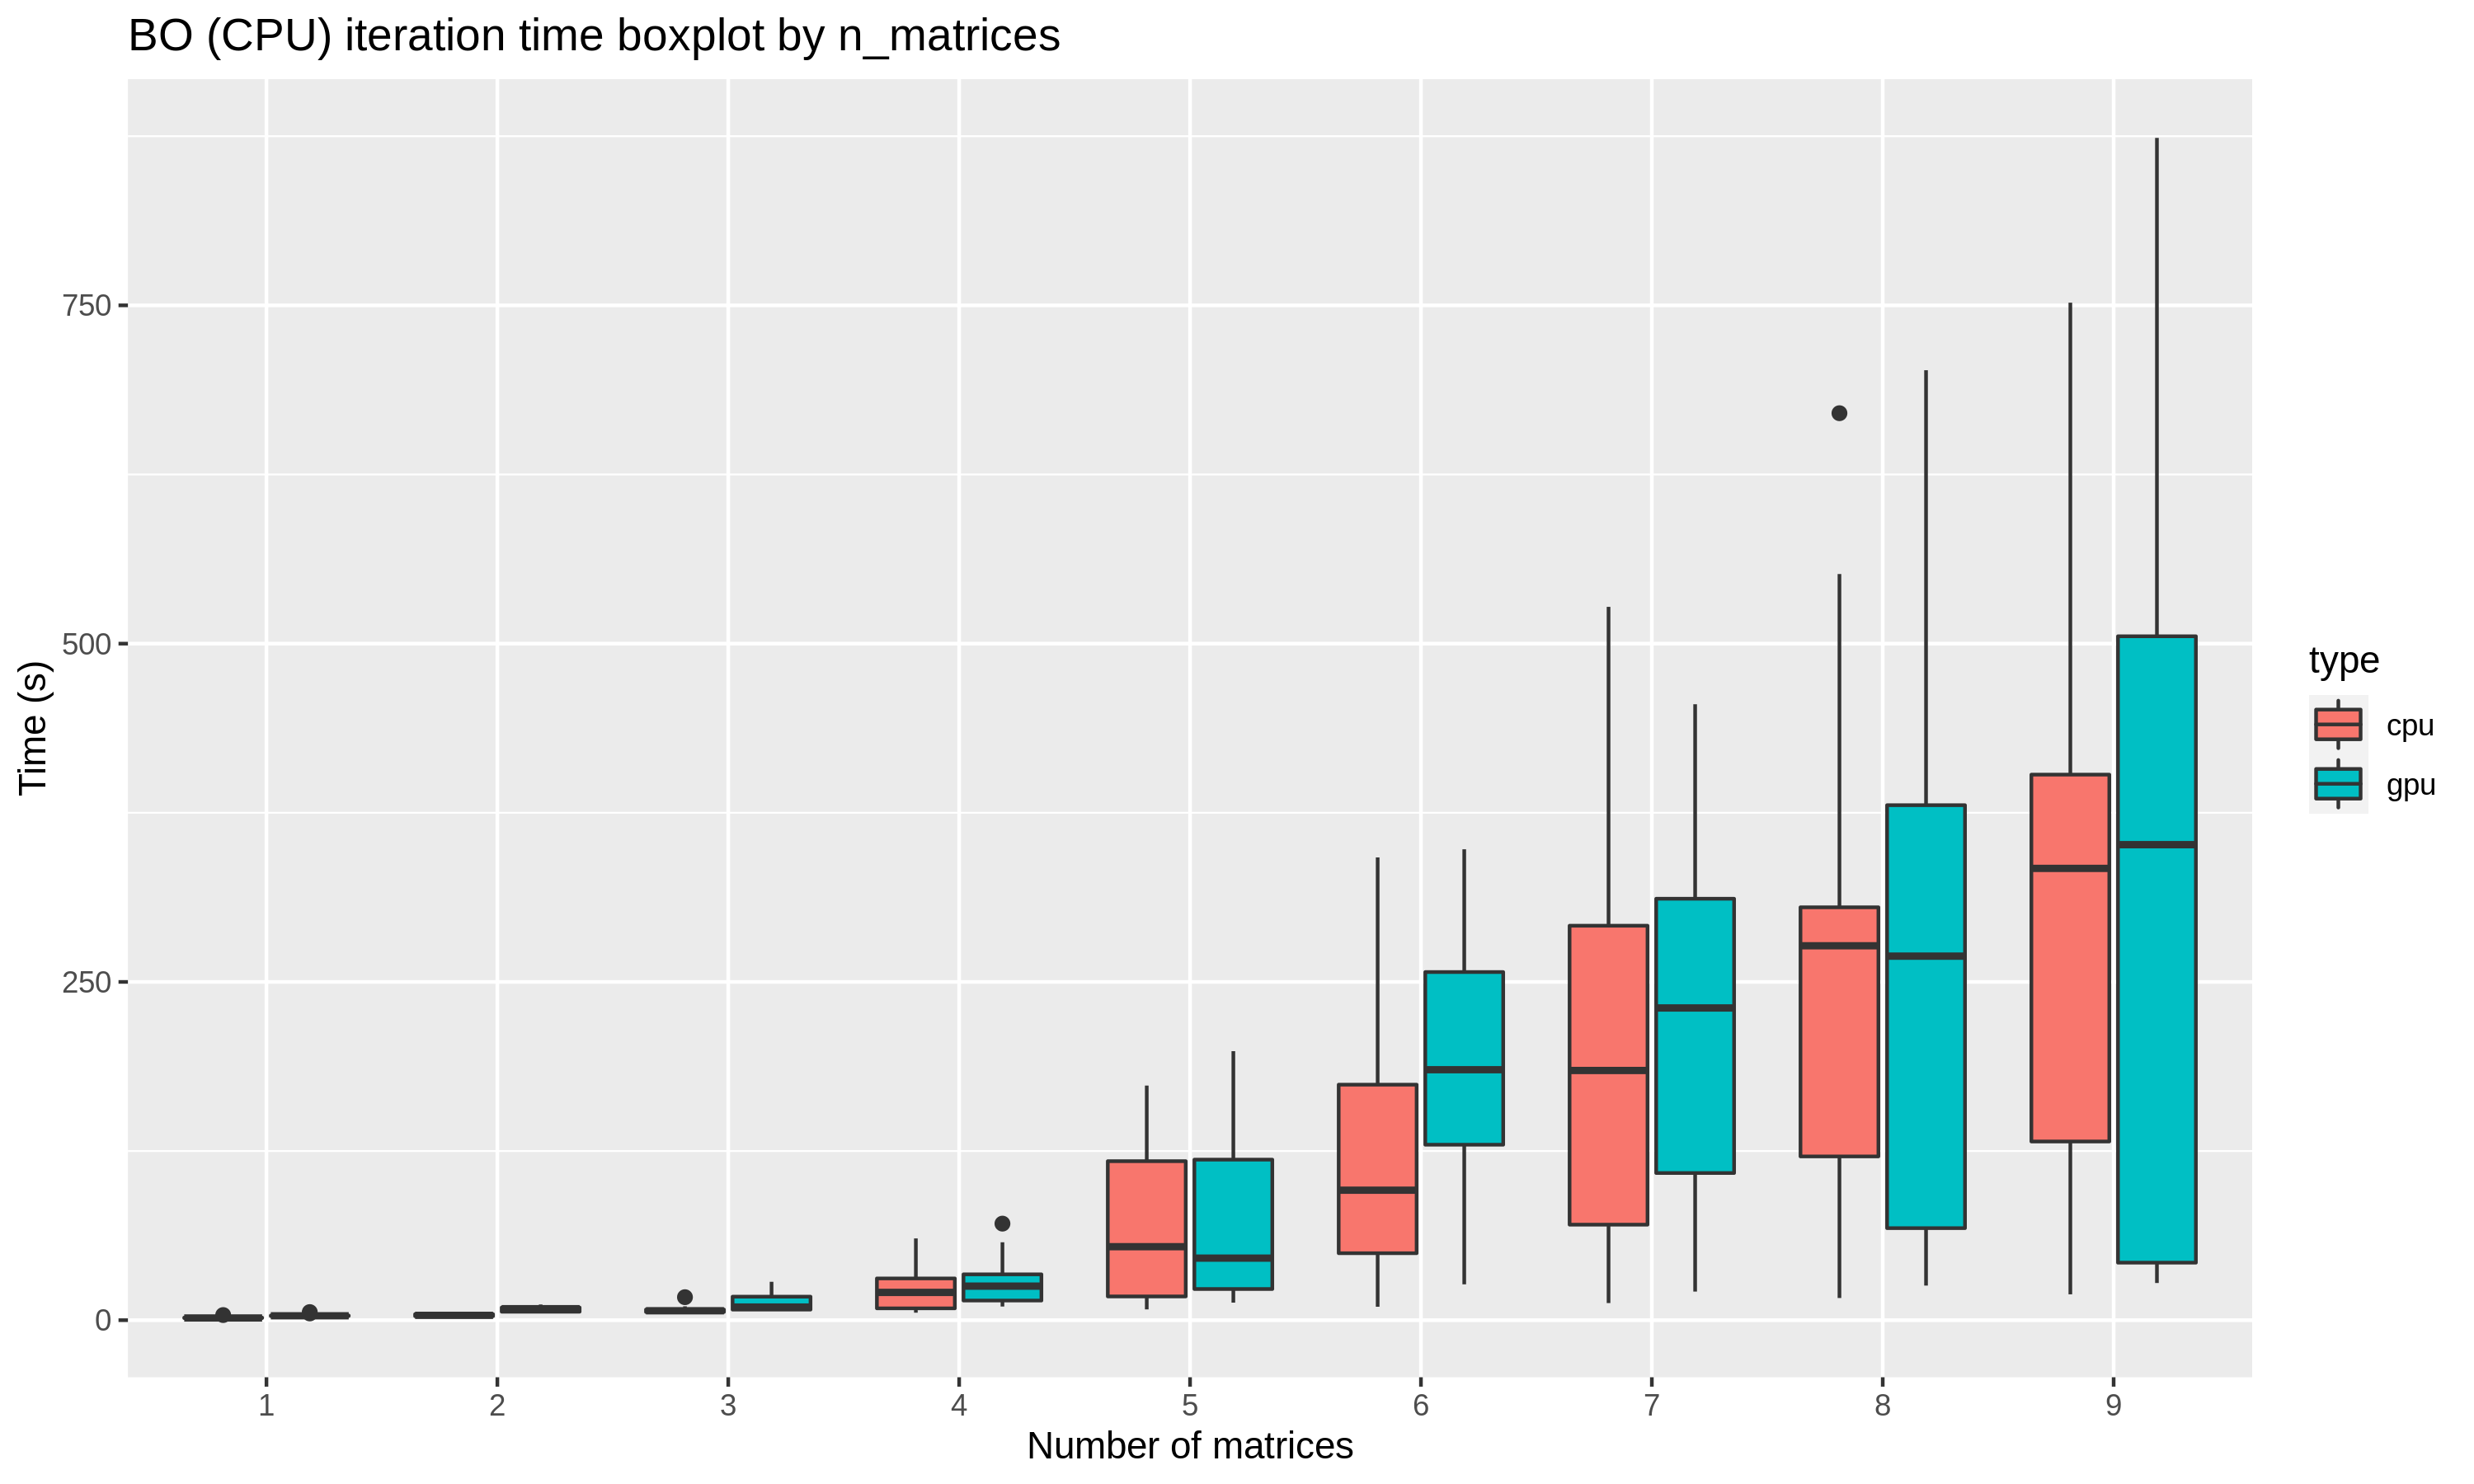
\includegraphics[width=\textwidth]{figures/bo_boxplot}
\decoRule
\caption[BO iteration time boxplot]{BO iteration time boxplot by number of matrices and computation paradigm. No significant differences between CPU/GPU are apparent; the higher values with 6 matrices using the GPU is likely to be due to chance.}
\label{fig:bo_boxplot}
\end{figure}

\begin{figure}[h!]
\centering
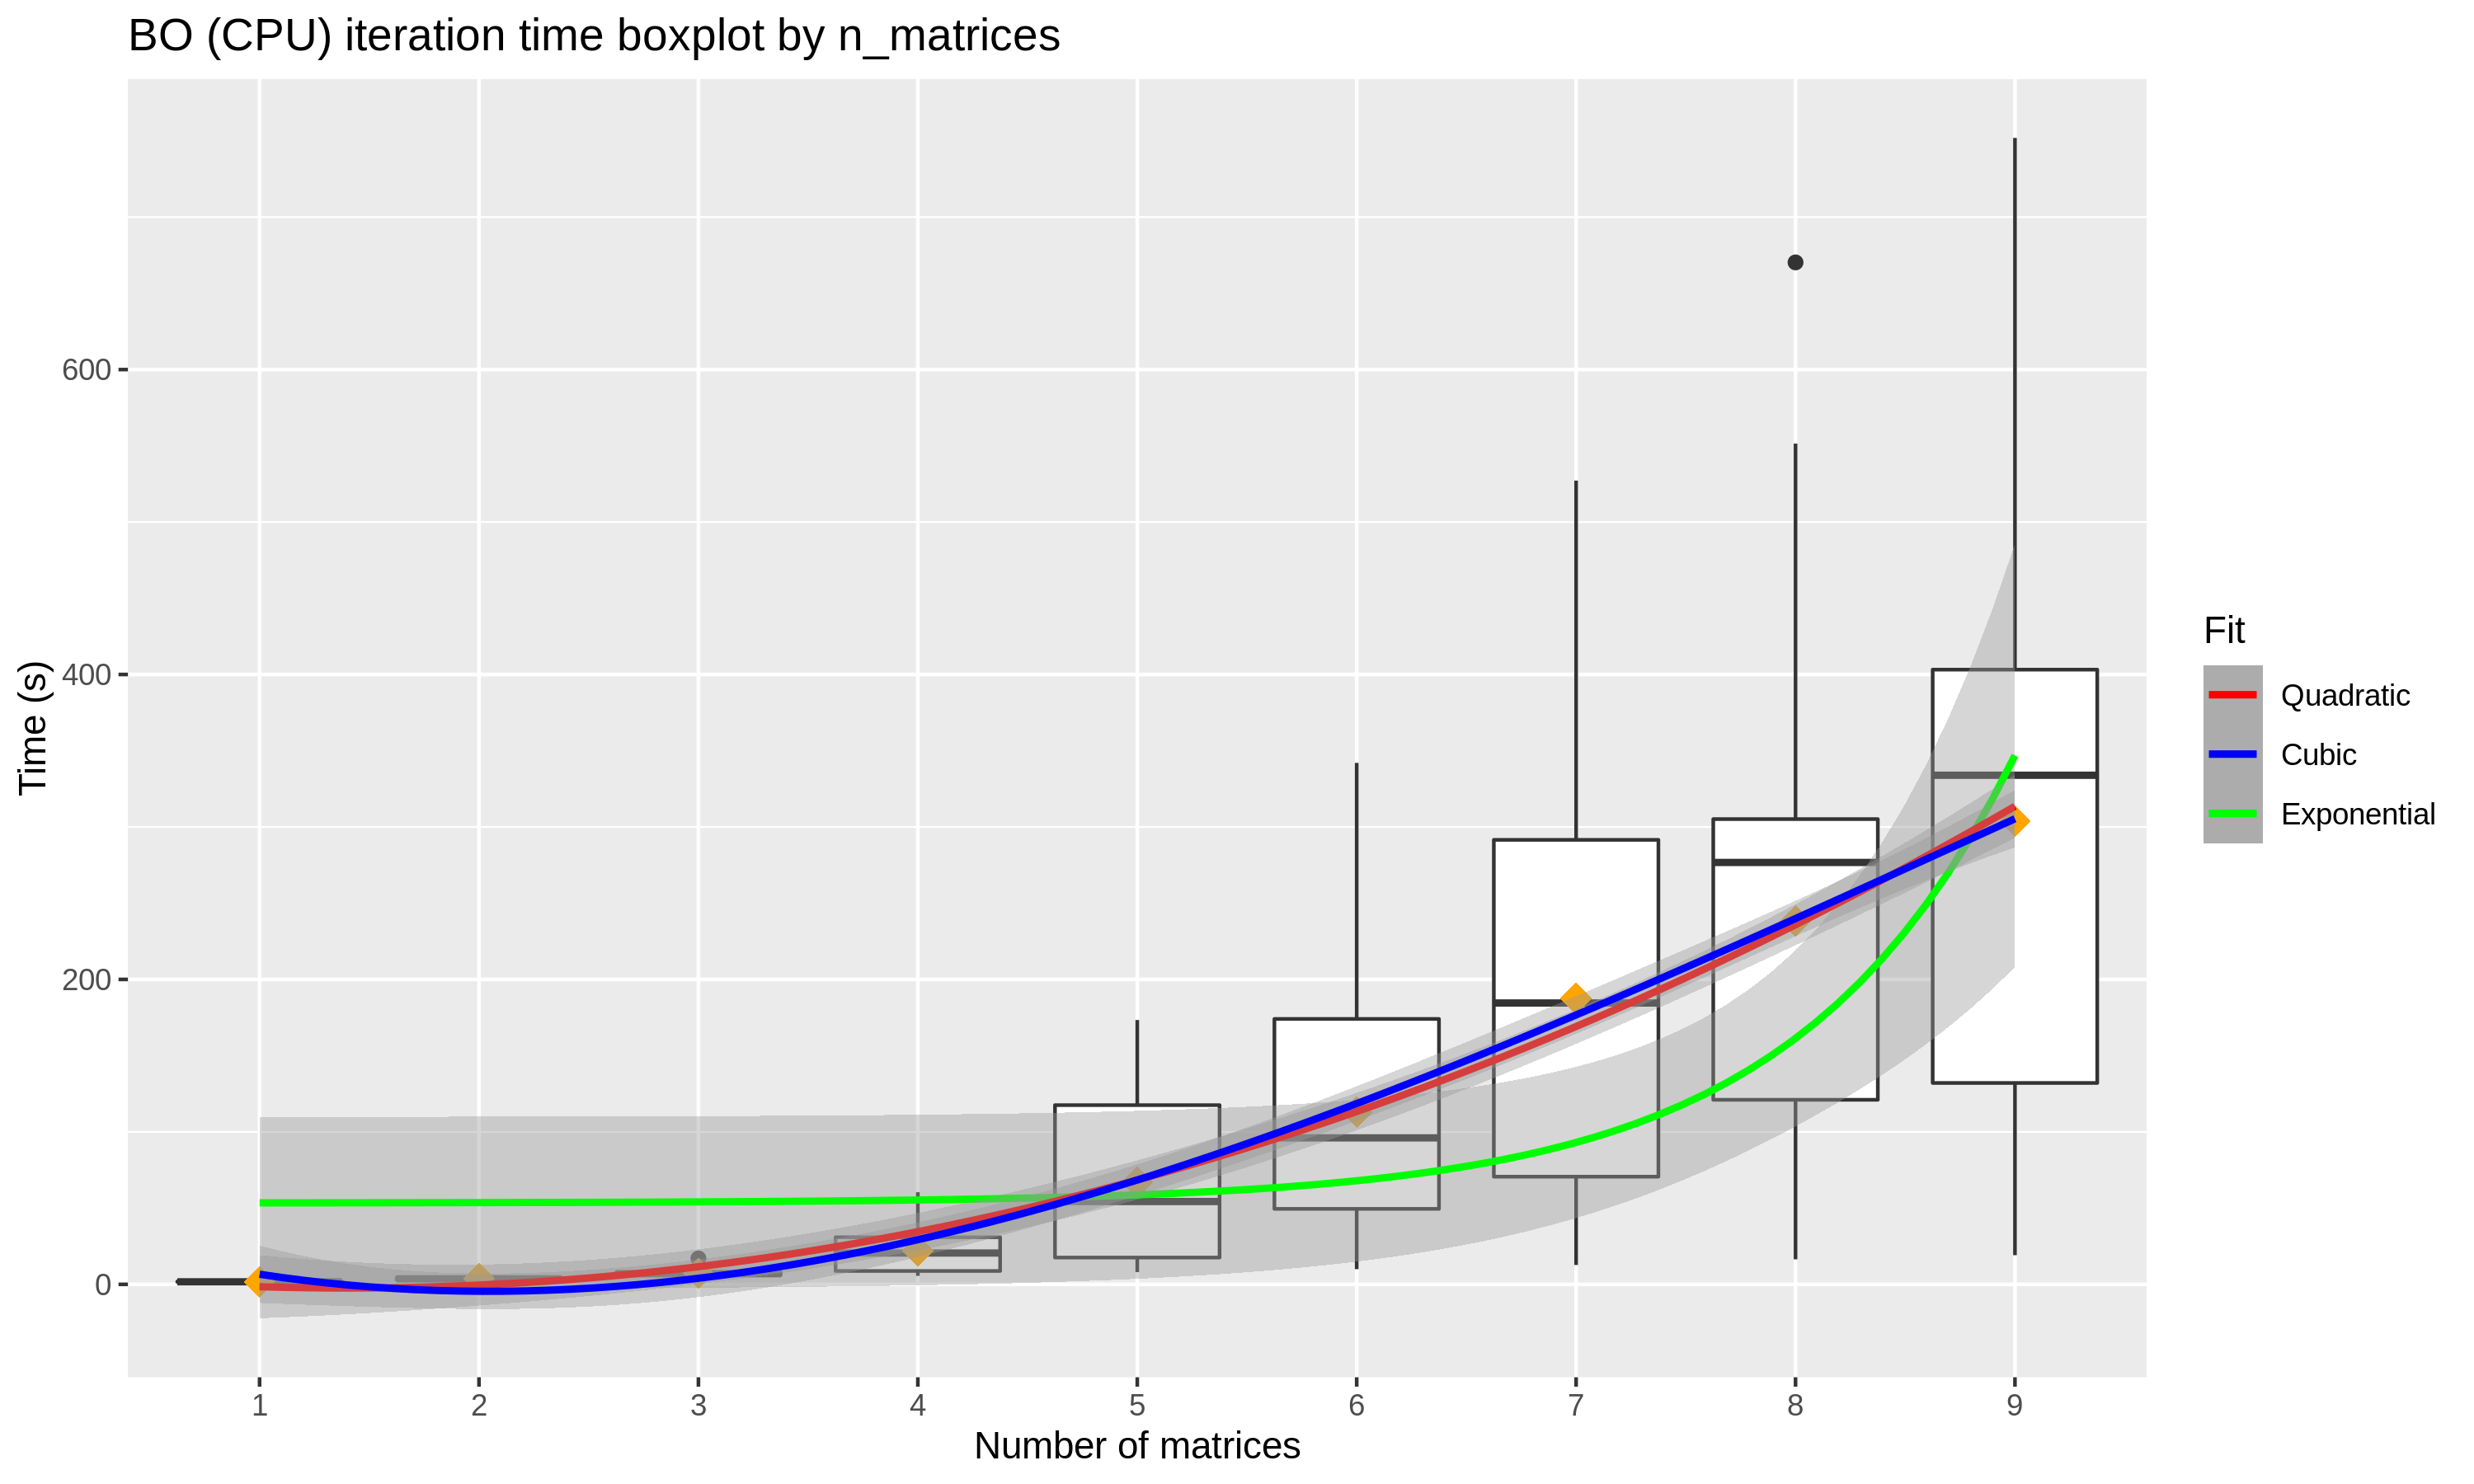
\includegraphics[width=\textwidth]{figures/bo_boxplot_cpu}
\decoRule
\caption[BO iteration time boxplot (CPU)]{CPU BO iteration time boxplot by number of matrices using the CPU with the means displayed in orange. As the number of matrices (and hence dimensions in the search space) increase the iteration time follows a quadratic trend instead of the expected exponential curve (?).}
\label{fig:bo_boxplot_cpu}
\end{figure}

\begin{figure}[h!]
\centering
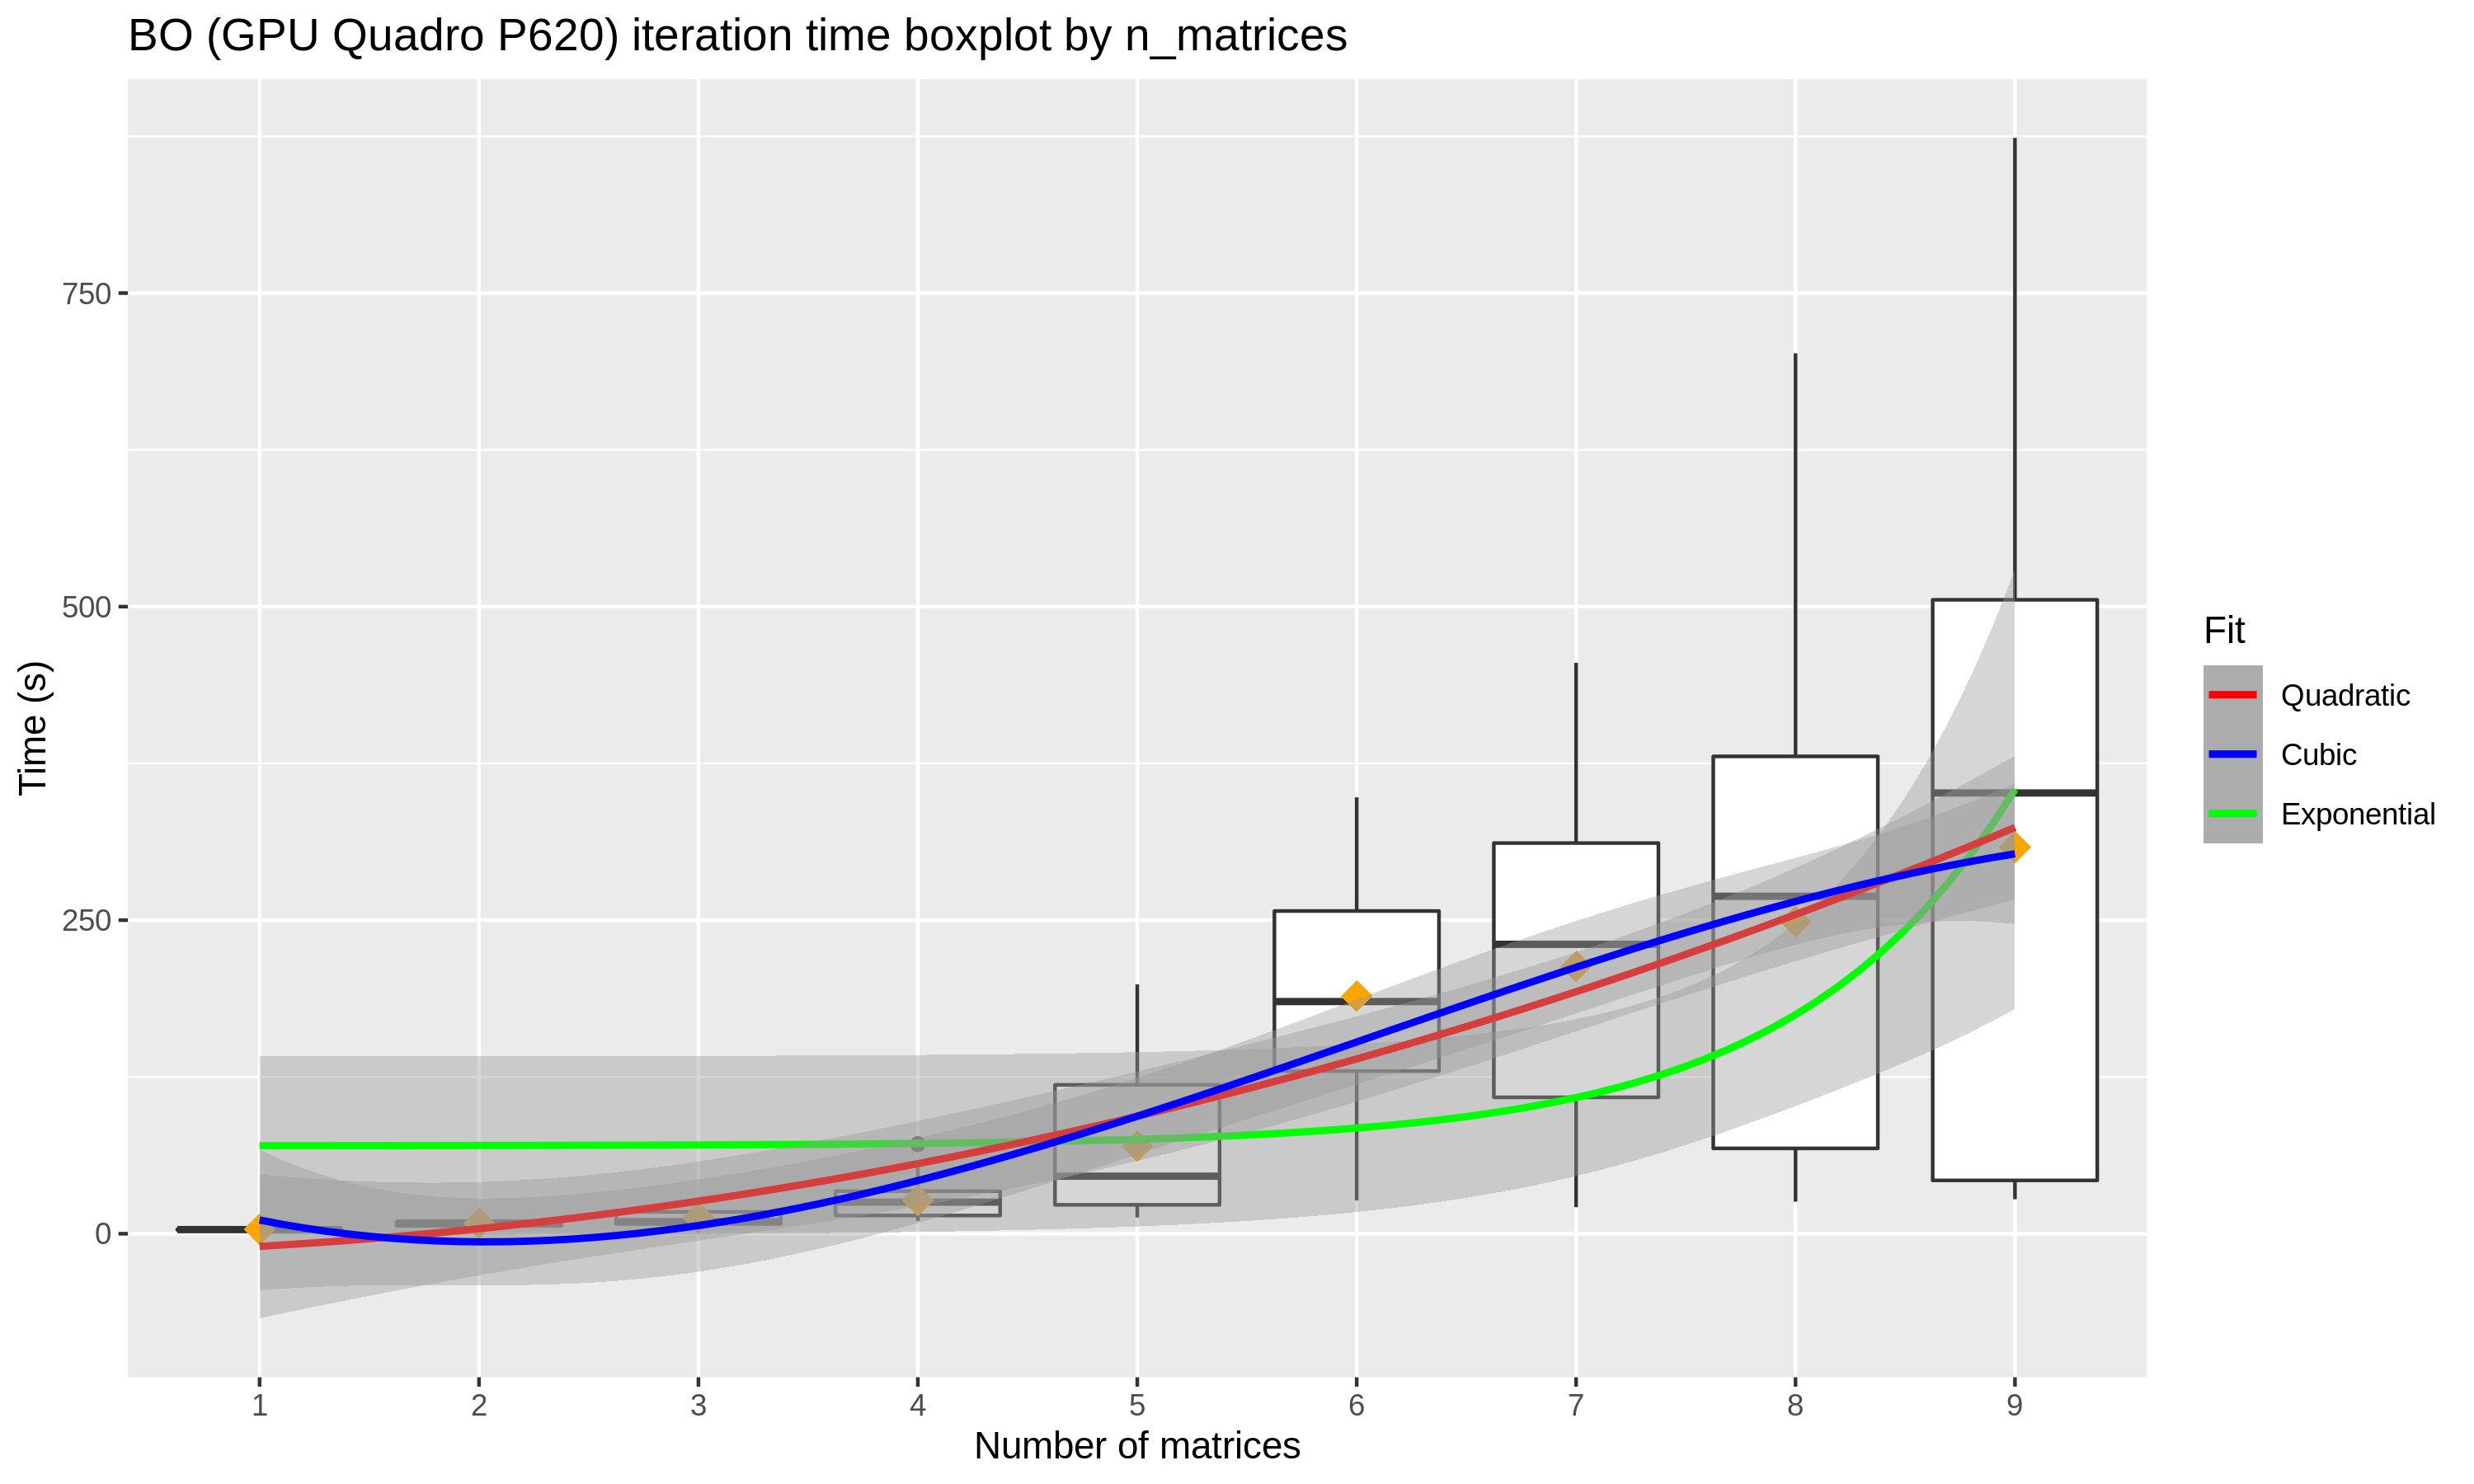
\includegraphics[width=\textwidth]{figures/bo_boxplot_gpu}
\decoRule
\caption[BO iteration time boxplot (GPU)]{GPU BO iteration time boxplot by number of matrices using the CPU with the means displayed in orange. As the number of matrices (and hence dimensions in the search space) increase the iteration time follows a quadratic trend instead of the expected exponential curve (?).}
\label{fig:bo_boxplot_gpu}
\end{figure}